\documentclass[pdftex,english,11pt,parskip=half]{scrartcl}
\usepackage{palatino}
\usepackage{mathpazo}
\usepackage[margin=0.7in]{geometry}
%\usepackage{parskip}
\usepackage[compact]{titlesec}
\usepackage{amsmath,amssymb}
\usepackage{graphicx}
\usepackage{babel}
\usepackage{framed}
\usepackage{wrapfig}
\usepackage{subfig}
\usepackage{sidecap}
\usepackage[labelfont=bf,font=small,format=plain]{caption}
\usepackage{doi}
\usepackage{booktabs}
\usepackage{longtable}
\usepackage{multirow}
\usepackage[table]{xcolor}
\usepackage{wrapfig}
\usepackage{colortbl}
\usepackage{pdflscape}
\usepackage{tabu}
\usepackage{threeparttable}
\usepackage{threeparttablex}
\usepackage{array}
\usepackage[normalem]{ulem}
\usepackage{makecell}
\usepackage{float}
%\usepackage[authoryear]{natbib}
\usepackage[numbers]{natbib}
\usepackage{url,hyperref,color}
\usepackage{rotating}
\usepackage{lscape}
\definecolor{darkblue}{rgb}{0.0,0.0,0.75}
\hypersetup{colorlinks,breaklinks,
            linkcolor=darkblue,urlcolor=darkblue,
            anchorcolor=darkblue,citecolor=darkblue}
\newcommand{\fixme}[1]{{\color{red} #1}}
\renewcommand\thesection{\Alph{section}}
\renewcommand{\familydefault}{\sfdefault}
\newcommand{\tabitem}{~~\llap{\textbullet}~~}
\begin{document}
\addtokomafont{section}{\large}
\def\bf{\normalfont\bfseries}
\pagestyle{empty}

\section*{Research Education Program Plan}

\section{Significance}
\vspace{-0.1in}

Current focal points of NIH-funded biomedical research include translational
medicine, big data analyses of genomic, proteomic, and metabolomic experiments,
and team science \cite{}, all of which rely on the generation, sharing, and
integration of high-quality experimental data that may be used and re-used in
multiple types of analysis and visualization platforms. The NIH Strategic Plan
for Data Science \cite{} emphasizes the critical need to capitalize on this
emerging ecosystem of data, and includes the need to address multiple practical
issues related to data storage, management, accessibility, and usablility.
However, consideration of the current sources of much of this data from
individual bench scientists and academic research groups, leads to the 
recognition that a large amount of biomedical data collection is in the form 
of commercial or open source spreadsheets that contain sometimes complex 
organizational
patterns of quantitative and qualitative tables, charts, graphs, notes and other
figures, embedded black-box statistical calculations, and mixtures of
experimental data types and units. Further, it is widely known and discussed
among data scientists, mathematical modelers, and statisticians \cite{}, that
there is a frequent need disgard, transform, and reformat sometimes large
amounts of this primary data and meta-data. While such ``data cleaning'' is
necessary for it's use in the advanced and developing data tools, it is often
conducted by the data-scientist with minimal or no communcation with those who
generated the data. From our experience with drug and vaccine development for
infectious diseases, \textbf{we have identified this step of data recording and
pre-processing as a potential critical point of failure for reproducible
research results.} In this proposal, we provide a solution to mitigate such
potential failures by using the R programming language and the concept of "tidy"
data stuructures, together with a set of training modules that are aimed at the
laboratory bench scientists whose attention is rather to their experimental
technique and collection of accurate data, and who may have little or no
background in the use of general purpose software tools.

While this proposal uses examples from microbiology and immunology experiments,
the collection of primary data in a flexible, open source, transpararent, 
and reproducible format, which can be kept in it's primary state without the 
need for additional modification, is a solution that extends thoughout
large and small scale biomedical science projects.  Figure () below shows an 
example workflow of such a comprehensive experimental data and quantitative 
analysis framework, and indicates our specific focus, highlighting it's 
critical place in such an analysis framework.

\section{Innovation} \vspace{-0.1in}

To disseminate the training materials we develop, \textbf{we will use the
innovative \textit{bookdown} framework \cite{xie2016bookdown} to structure and
publish all of our training materials as a free and open online book}. The
\textit{bookdown} framework has been available for a little over two years and
extends the principles of \textit{rmarkdown} to allow users to create attractive
online books that integrate programming code and text. This format allows
authors to efficiency create books with many coding examples---code and its
output does not need to be copied and pasted into a document, but instead can be
automatically generated each time the book is edited. Also, since the book is
created by executing those code examples, regularly test that all code remains
free of bugs created by changes in dependencies (e.g., updates to R packages
used in the code) \cite{xie2016bookdown}. Through this innovative framework, we
will be able to create a searchable online book that weaves R code into the text
and that can include embedded tutorial videos, active weblinks to online
references, and computationally reproducible practice examples and exercises
(Figure \ref{fig:prototype}). While relatively new, this framework has proven
itself reliable and effective---it serves as the framework for several extremely
popular and highly-accessed books on R programming, including \textit{R for Data
Science} [ref]. 

\begin{figure}[t] 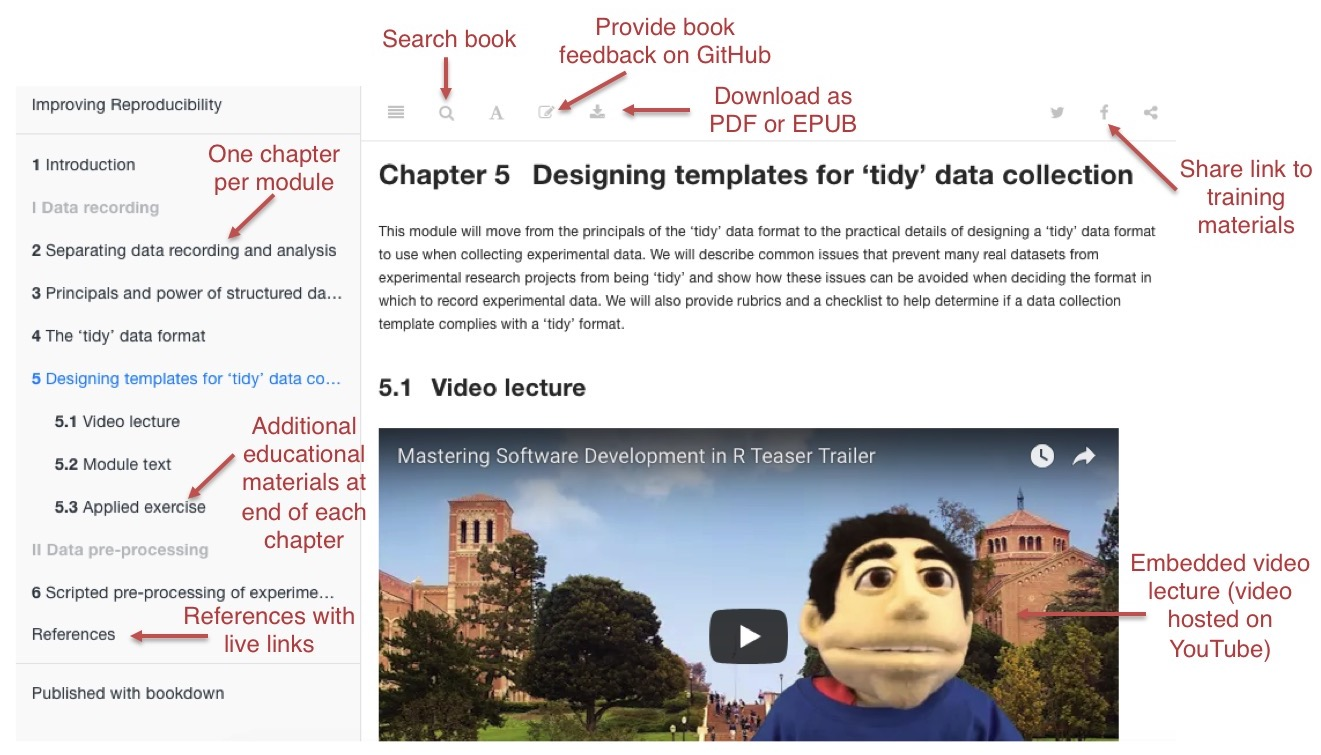
\includegraphics[width =
\textwidth]{figures/book_prototype.jpg} \caption{Prototype of online course
book, with features highlighted.} \label{fig:prototype} \end{figure}

Dr. Anderson (PI) was an early adopter of the \textit{bookdown} framework. Since
it became available, she has used it to create two \textit{bookdown}-based
books: the \textit{R Programming for Research} online coursebook, which she uses
as a joint textbook and website for the \textit{R Programming for Research}
course she teaches each fall at Colorado State University, and \textit{Mastering
Software Development in R}, which she co-wrote with Dr. Roger Peng as a manual
for developing advanced R programming skills and which has been downloaded by
over 14,000 people from LeanPub (see letter from Dr. Peng). Dr. Anderson served as one of the six
reviewers---along with R programming experts Jan de Leeuw, Karl Broman, Michael
Grayling, Daniel Kaplan, and Max Kuhn---for \textit{bookdown: Authoring Books
and Technical Documents with R Markdown} \cite{xie2016bookdown}.

\textbf{The use of this framework will help us effectively reach a large
audience in need of training materials for improving the reproducibility of data
recording and pre-processing in biomedical research.} We will be able to freely
post this book online using the Git Pages feature of GitHub, as we have done
with previous books created with the same framework. This will allow anyone to
freely access this content online, and to explore the module contents to find
the set of modules that best suits their immediate training needs. The
book-style format makes the content easy to navigate through both its use of
sections and chapters to group material and through its embedded search
functionality (Figure \ref{fig:prototype}). Further, researchers will be able to
download the book as either a PDF or EPUB file, to use as a reference as they
continue learning to implement reproducibility tools in their research projects.
[More about this.]

We will publish the book's code openly online through GitHub from the beginning
of our development of the training materials, as well as publish the current
version of materials as the online book. \textbf{By making the training
materials available from day one, as they are developed, we will be able to
attract early users to help disseminate the material as it evolves and also be
able to get early feedback on the content as it is developed.} Once the online
book is developed, we will be able to submit a static version of it to be posted
on the homepage of the \textit{bookdown.org} website [ref], which will serve as
another way for trainees to find and access the materials.

\section{Approach---Proposed Research Education Program}

\textbf{Project goals and objectives.} Our project's primary goal is to develop
training modules that address the needs of laboratory-based biomedical
researchers seeking to improve reproducibility, especially of experimental data
recording and pre-processing, in their research projects. The expected result of
this project is an online book that contains twenty short training modules as separate
chapters, with video lectures, written text, and additional educational
materials collected within each module's chapter. We consider it critical that
these training materials be clear, relevant, and useful to a key audience of
biomedical scientists whose primary research activities focus on laboratory
research, rather than data analysis or statistics. To help us achieve this goal,
our team includes three co-investigators from this key audience who will play an
early and continuing role in developing and refining the training materials for
this audience, and our plan includes intensive user testing of the developing
materials on several groups of pilot testers from this audience. Our
co-investigators' network of connections in Microbiology and Immunology will
help us widely disseminate these materials to our target audience, as will the
free, online format of the materials and presenting the materials at national
and international Microbiology and Immunology conferences in the second and
third years of the project.

\begin{itemize}
\item ``Without formal requirements for continuing education, the most effective solutions may be to develop educational resources that are accessible, easy-to-digest and immediately and effectively applicable to research (for example, brief, web-based modules for specific top- ics, and combinations of modules that are customized for particular research applications). A modular approach simplifies the process of iterative updating of those materials. Demonstration software and hands-on examples may also make the lessons and implications par- ticularly tangible to researchers at any career stage" \cite{munafo2017manifesto}\item ``Studies of statistical power persistently find it to be below (sometimes well below) 50\%, across both time and the different disciplines studied [2,35,36]. Low statistical power increases the likelihood of obtaining both false-positive and false-negative results [2], meaning that it offers no advantage if the purpose is to accumulate knowledge. Despite this, low-powered research persists because of dysfunctional incentives, poor understanding of the consequences of low power, and lack of resources to improve power. Team science is a solution to the latter problem---instead of relying on the limited resources of single investigators, distributed collaboration across many study sites facilitates high-powered designs and greater potential for testing generalizability across the settings and populations sampled. This also brings greater scope for multiple theoretical and disciplinary perspectives, and a diverse range of research cultures and experiences, to be incorporated into a research project." \cite{munafo2017manifesto}
\item ``Multi-centre and collaborative efforts have a long and successful tradition in fields such as randomized controlled trials in some areas of clinical medicine, and in genetic association analyses, and have improved the robustness of the resulting research literatures. Multi-site collaborative projects have also been advocated for other types of research, such as animal studies [41--43], in an effort to maximize their power, enhance standardization, and optimize transparency and protection from biases. The Many Labs projects illustrate this potential in the social and behavioural sciences, with dozens of laboratories implementing the same research protocol to obtain highly precise estimates of effect sizes, and evaluate variability across samples and settings [44,45]. It is also possible, and desirable, to incorporate a team science ethos into student training " \cite{munafo2017manifesto}
\item ``According to a U.S. National Science Foundation (NSF) subcommittee on replicability in science (9), 'reproducibility refers to the ability of a researcher to duplicate the results of a prior study using the same materials as were used by the original inves- tigator. That is, a second researcher might use the same raw data to build the same analysis files and implement the same statistical analysis in an attempt to yield the same results.... Reproducibility is a minimum necessary condition for a finding to be believable and informative.' ... Reproducibility defined in this way mainly addresses issues of trust that data and analyses are as represented. The definition does not specify to what extent deviations are acceptable. Such reproducibility does not add new evidential weight, although greater subjective weight is often accorded to evidence that is more highly trusted. New evidence is provided by new experimentation, defined in the NSF report as 'replicability,' which refers to 'the ability of a researcher to duplicate the results of a prior study if the same procedures are followed but new data are collected.'" \cite{goodman2016does}
\item ``How can we dramatically scale up data science education in the short term? One approach that we have taken is through massive online open courses (MOOCs). The Johns Hopkins Data Science Speciali- zation (jhudatascience.org) is a sequence of nine courses covering the full spectrum of data science skills from formulating quan- titative questions, to cleaning data, to sta- tistical analysis and producing reproducible reports. Thus far, we have enrolled more than 1.5 million students in this Specializa- tion. A complementary approach is crowd- sourced short courses such as Data and Soft- ware Carpentry (software-carpentry.org) that have addressed the extreme demand for data science knowledge on a smaller scale. However, simply increasing data analytic literacy comes at a cost. Most scientists in these programs will receive basic to moderate training in data analysis, creating the potential for producing individuals with enough skill to perform data analysis but without enough knowledge to pre- vent mistakes.
To improve the global robustness of scientific data analysis, we must couple education efforts with the identification of data analytic strategies that are most re- producible and replicable in the hands of basic or intermediate data analysts. Statisti- cians must bring to bear their history of developing rigorous methods to the area of data science." \cite{leek2015opinion}
\item ``Novices program differently than experts [26] and need different approaches or tools. If you ask a professional programmer to iterate over a list of integers and produce the average, they can write the code within seconds, using stored knowledge of the exact pattern required. Novices will approach this problem totally differently: they need to remember the syntax for the different parts, know how to iter- ate over a list, know how to use an accumulator variable, and so on.
Novices may need to spend time thinking about an algorithm on paper (something expert programmers rarely need, as they have usually memorised most common algorithmic pat- terns). They may need to construct examples in guided steps. They may struggle to debug. Debugging usually involves contrasting what is happening to what should be happening, but a novice’s grasp on what should be happening is usually fragile.
Novices do not become professionals simply by doing what professionals do at a slower pace. We do not teach reading by taking a classic novel and simply proceeding more slowly. We teach by using shorter books with simpler words and larger print. So in programming, we must take care to use small, self-contained tasks at a level suitable for novices, with tools that suit their needs and without scoffing." \cite{brown2018ten}
\item ``Our final tip for teaching programming is that you don’t have to program to do it. Faced with the challenges of learning syntax, semantics, algorithms, and design, examples that seem small to instructors can still easily overwhelm novices. Breaking the problem down into smaller sin- gle-concept pieces can reduce the cognitive load to something manageable." \cite{brown2018ten}
\end{itemize}

\subsubsection*{Proposed training modules}

\begin{quotation} ``State the \textbf{goals for education} and \textbf{justify
the area of training} selected for module development in terms of its
\textbf{relevance and potential impact} on improving the development of skills
and knowledge important for conducting rigorous and reproducible research.
Describe the \textbf{subject material} to be covered. The \textbf{length} of the
proposed training module should be explained in terms of \textbf{scope and depth
of coverage} of the subject matter.  In addition, \textbf{how the research
education will be utilized by trainees or investigators} should be
described---for example, a module on how to avoid confirmation bias to be taken
by all beginning laboratory workers, or a module on appropriate design of animal
studies to be taken immediately prior to beginning such work." \end{quotation}

Our emphasis on primary experimental data collected and recorded as a data
structure, specifically the innovative "tidy" data format developed within the R
statistical programming environment, and presented in an innovative e-book
format

[A paragraph on why we, specifically, passionately think that these training
modules would address a key need.] Our team combines experts in R programming
(Anderson, Lyons) with a group of biomedical researchers (Gonzalez-Juarrero,
Henao-Tamayo, and Robertson) who have, collectively, spent decades in
laboratory-based research to improve understanding of tuberculosis and other
diseases. We met as faculty members of the same College at Colorado State
University, and since have discovered how many of the tools that Drs. Anderson
and Lyons teach and use to improve the reproducibility of \textit{data analysis}
for biomedical research could substantially improve reproducibility and
trasparency in the laboratory-based biomedical research projects of Drs.
Gonzalez-Juarrero, Henao-Tamayo, and Robertson at the stages of \textit{data
recording} and \textit{data pre-processing}. Over the past year, we have begun
to work together to do this within our own research projects: for example, in
Fall 2017 Dr. Gonzalez-Juarrero attended Dr. Anderson's (PI) course in \textit{R
Programming for Research} and has brought the ideas and techniques back to her
research laboratory, in Fall 2017 Dr. Lyons worked with Dr. Anderson to bring in
real tuberculosis drug development data to use in the final group project in Dr.
Anderson's R Programming course, and in Spring 2018 Dr. Henao-Tamayo and Dr.
Anderson began co-advising a graduate student with the aims of implementing
open-source tools for pre-processing flow cytometry in Dr. Henao-Tamayo's
laboratry. Collectively, we are passionate about the idea that
\textbf{open-source tools can be used to bring substantial improvements to
reproducibility of data recording and pre-processing in laboratory-based
research}, and yet we are also able to recognize the key barriers in
implementing these tools in this setting, as well as in training
laboratory-based researchers in how to use these tools, and why existing free
training materials have, to date, been limited in meeting these needs for the
key audience of laboratory-based biomedical researchers. 

[Paragraph on why we are focusing on data recording and data pre-processing.]
Many excellent free training resources exist to improve the computational
reproducibility of biomedical research. However, most of these
materials---including some developed by Dr. Anderson for her open online and
CSU-based courses in R programming [refs]---target researchers at the stage of
\textit{data analysis}, and provide much less guidance on the principles and
techniques to improve reproducibility of the earlier steps of
\textbf{experimental data recording} and \textbf{experimental data
pre-processing}. In this project, we will create training modules to fill this
gap. [More on this, ideally with some references to the importance of
reproduciblity in these steps.]

[A paragraph on who our key audience is and why we are focusing on that
audience.] A key aim is to make these modules \textbf{accessible and useful to
our target audience, laboratory-based researchers}. Three of the Co-Is on our
team (Gonzalez-Juarrero, Henao-Tamayo, and Robertson) represent this key
audience. [Why it is so important to develop these training materials for this
audience.]

[A paragraph about how we plan to focus on this audience] We plan to make these
modules accessible and useful to our target audience, laboratory-based
researchers by including examples from real microbiology and immunology research
projects and by piloting the training modules among laboratory-based biomedical
researchers. Our training materials will provide resources that can be used by
this audience of researchers at a variety of levels, from undergraduate students
to principal investigators, with a modular design that will allow a trainee to
use the subset of modules the best meets his or her immediate needs.

[A paragraph on how our training materials will fit in with the training
materials developed under previous rounds of this grant.]

We aim to create training modules that will show laboratory-based biomedical
researchers how simple computational reproducibility principles can improve
biomedical research reproducibility at the stages of data recording and
preprocessing and teach them how to implement these principles in their
laboratories. The importance of computational reproducibility of scientific
research is increasingly recognized by scientists, journals, and funding
agencies, with such ``computationally reproducible" research requiring that all
data and code for a research project be available and that this data and code
can be used to regenerate study findings either by the original researcher or by
other researchers \cite{ellis2018share, ram2013git}. Among our team, we have
found that there are many common existing practices---including use of
spreadsheets with embedded macros to concurrently record and analyze
experimental data, unstructured [too strong?] management of project files,
reliance on proprietory, vendor-supplied point-and-click software for data
pre-processing---that can interfere with the transparency, reproducibility, and
efficiency of the kind of research they conduct. [Some more about how we're not
the first people to notice that this is a problem for reproducibility / rigor.] 

We propose to develop two collections of modules, \textbf{Improving the
Reproducibility of Experimental Data Recording} and \textbf{Improving the
Reproducibility of Experimental Data Pre-Processing}. Our team has worked
together to create a curriculum of training modules that we believe will help
fill an important training gap for laboratory-based biomedical researchers
(Tables \ref{tab:content_one} and \ref{tab:content_two}). The first sequence,
\textbf{``Improving the Reproducibility of Experimental Data Recording"; Table
\ref{tab:content_one}}, will explore the pitfalls of combining experimental data
recording and analysis within macro-enabled spreadsheets, explain the power
structured data formats for recording data, describe how reproducibility can be
improved by using a single structured directory to store all research project
files, and demonstrate the use of version control to maintain single, current
versions of all files while saving a history of all file changes. The second
sequence, \textbf{``Improving the Reproducibility of Experimental Data
Pre-Processing"; Table \ref{tab:content_two}}, will focus on improving the
reproducibility of experimental data pre-processing steps, like gating for flow
cytometry data and peak finding / quantifying for mass spectrometry data.
Training materials will explain how the use of code scripts for these steps
dramatically improves reproducibility compared to using vendor-supplied
point-and-click software and will introduce trainees to popular R software for
this pre-processing. This sequence will include advice on reproducible data
pre-processing protocols and how to create them using literate programming tools
(\textit{Rmarkdown}).

Each module will fall into one of three categories for teaching reproducibility:
(1) principals; (2) implementation; and (3) case study examples. ``Principals"
modules will be programming-language agnostic, while ``Implementation" modules
will focus on tools available through the popular open source R software and its
RStudio interface. Working with the biomedical laboratory-based co-investigators
on our team, we will ensure that these modules and the examples used in them are
approachable and useful to researchers with limited computational training. We
have divided the content into modules in a way that will allow \textbf{trainees
and investigators at any level} to create their own ``tracks" by selecting
relevant subsets of the modules to complete, and potentially combining this
content with other training modules available through the NIH's [Clearinghouse]
[ref]. Table \ref{tab:tracks} gives a few examples of how different trainees
could create and follow their own ``track" of the material.

For many of the barriers we identified to reproducibility at these stages of
research, a simple fix exists. Our team has worked together to craft a list of
specific topics (Tables \ref{tab:content_one} and \ref{tab:content_two}) we aim
to address with these modules so that they will offer training in a collection
of principles and techniques that tackle barriers to reprodubility with
straightforward fixes, but which we have found are still very common in
biomedical laboratory-based research programs, including those here at Colorado
State University. We have identified several easy-to-address barriers to
computational reproducibility at two stages of biomedical research: experimental
data recording and experimental data pre-processing.

\begin{itemize}
\item ``From our experience in the Leek group (where we work with a large number of collaborators to analyze data) and from conversations with other statisticians, the primary source of delay in the speed of returning results to collaborators is the con- dition of the data when they arrive." \cite{ellis2018share} `
\item `Consistent data sharing reduces the likelihood of errors during analysis and also decreases analysis turnaround time [when collaborating with statisticians."  \cite{ellis2018share} 
\item ``When a researcher turns over a properly tidied dataset, it dramatically decreases the workload on the statistician and minimizes the likelihood of errors during analysis."  \cite{ellis2018share}
\item ``Unquestionably, a significant contribu- tor to failure in oncology trials is the qual- ity of published preclinical data. Drug development relies heavily on the literature, especially with regards to new targets and biology. Moreover, clinical endpoints in can- cer are defined mainly in terms of patient survival, rather than by the intermediate endpoints seen in other disciplines (for example, cholesterol levels for statins). Thus, it takes many years before the clinical appli- cability of initial preclinical observations is known. The results of preclinical studies must therefore be very robust to withstand the rigours and challenges of clinical trials, stemming from the heterogeneity of both tumours and patients. The scientific community assumes that the claims in a preclinical study can be taken at face value — that although there might be some errors in detail, the main message of the paper can be relied on and the data will, for the most part, stand the test of time. Unfor- tunately, this is not always the case. Although the issue of irreproducible data has been discussed between scientists for decades, it has recently received greater attention (see go.nature.com/q7i2up) as the costs of drug development have increased along with the number of late-stage clinical-trial failures and the demand for more effective therapies." \cite{begley2012drug}
\item ``Although the importance of multiple studies corroborating a given result is acknowledged in virtually all of the sciences (Fig. 1), the modern use of “reproducible research” was originally applied not to corroboration, but to transparency, with application in the com- putational sciences. Computer scientist Jon Claerbout coined the term and associated it with a software platform and set of proce- dures that permit the reader of a paper to see the entire processing trail from the raw data and code to figures and tables (4)." \cite{goodman2016does}
\item ``Statistical methods can be complex, and continue to evolve in many specialties, particularly novel ones such as omics. However, statisticians and methodologists are only sporadically involved, often leading to flawed designs and analyses.72 Much flawed and irreproducible work has been published, even when only simple statistical tests are involved. Investigators of one study73 examined the use of Fisher’s exact test in 71 articles from six major medical journals. When a statistician was a member of the team, the test was used more appropriately than when one was not. Data that are multidimensional (ie, contain many features) are particularly at risk of false positives and overfitting, particularly when analysed by inexperienced or untrained analysts. Problems with statistical analysis might not be identified in peer review, especially when the report is not assessed by a statistician or methodologist." \cite{ioannidis2014increasing}
\item ``Little evidence exists about the research training of laboratory scientists. The way that many laboratory studies are reported suggests that scientists are unaware that their methodological approach is without rigour (figure). Many laboratory scientists have insufficient training in statistical methods and study design. This issue might be a more important deficiency than is poor training in clinical researchers, especially for laboratory investigation done by one scientist in an isolated laboratory—by contrast, many people would examine a clinical study protocol and report." \cite{ioannidis2014increasing}
\item ``Statisticians and methodologists should be involved in all stages of research. This recommendation has been repeatedly discussed, mostly for clinical trials, but it applies to all types of studies. Enhancement of communication between methodologists and other health scientists is also important." \cite{ioannidis2014increasing}
\item These are early steps of the ``dry lab" part of an experiment.
\item ``We define reproducibility as the ability to recompute data analytic results given an observed dataset and knowledge of the data analysis pipeline. The replicability of a study is the chance that an independent experi- ment targeting the same scientific question will produce a consistent result (1). ... There have been some very public failings of reproduc- ibility across a range of disciplines from can- cer genomics (3) to economics (4), and the data for many publications have not been made publicly available, raising doubts about the quality of data analyses." \cite{leek2015opinion}
\item ``From a computational perspective, there are three major components to a reproducible and replicable study: (i) the raw data from the experiment are available, (ii) the statisti- cal code and documentation to reproduce the analysis are available, and (iii) a correct data analysis must be performed." \cite{leek2015opinion}
\item ``If we can prevent prob- lematic data analyses from being conducted, we can substantially reduce the burden on the community of having to evaluate an increasingly heterogeneous and complex population of studies and research findings. The best way to prevent poor data analysis in the scientific literature is to (i) increase the number of trained data analysts in the scientific community and (ii) identify sta- tistical software and tools that can be shown to improve reproducibility and rep- licability of studies." \cite{leek2015opinion}
\item ``In today’s technology-driven era of biological discovery, many biologists generate extremely large datasets, including high-throughput sequencing, proteomic and metabolomic spectra, and high-content imaging screens. Subsequently, biologists must overcome many challenges of incorporating computing into their standard procedures for data analysis, including installing and running software that is not 'point-and-click,' navigating at the command-line interface, comparing various analysis tools that supposedly perform the same tasks, establishing effective note-taking for their computing trials, and managing large datasets. Especially for trainees, it can be overwhelming to know how to begin to address these challenges. Providing a roadmap for workflow approach and management is likely to accelerate biologists’ skill-building in computing." \cite{shade2015computing}
\item ``Skills in computing can enhance biologists’ logic and capacity for experimental design, increase understanding and interpretation of results, and promote interdisciplinary science by building a shared vocabulary and experience with collaborators in computer science, bioinformatics, statistics, physics, and engineering. We’ve suggested a systematic roadmap for computing workflows for biologists, including considering the overarching goals of the workflow, taking an iterative approach to analysis, implementing reproducibility checkpoints, recording effective computing notes, and adopting a team approach to analysis." \cite{shade2015computing}
\item In fMRI: ``Although we aim for reproduction of results with other data and independent analysis methods, the first step is to ensure that results can be replicated within la- boratories. This seems an easy task, but it is in fact com- mon that results cannot be replicated after, say, a year or two, when the student or post-doc responsible for the analyses and the data management has left. Increasing our capacity to replicate the data analysis workflow has another crucial aspect: this will allow us to better docu- ment our work, and therefore communicate and share it much more easily. It is crucial that we remember that resources are limited, and part of our work is to make it easy for others to check and build upon our findings." \cite{pernet2015improving}
\item In fMRI: ``In computer science and related communities, a number of informatics tools and software are available (databases, control version system, virtual machines, etc.) to handle data and code, check results and ensure reproducibility. Neuroscientists working with functional MRI are, how- ever, largely from other communities such as biology, medicine and psychology. Because of the differences in training and the field of research, such informatics tools are not necessarily sufficient, and are certainly not fully ac- cessible to or mastered by all researchers. In this review, we address specifically the community of neuroscientists with little programming experience, and point to a num- ber of tools and practices that can be used today by any- one willing to improve his or her research practices, with a view to better reproducibility." \cite{pernet2015improving}
\item ``We define reproducibility as the ability of an entire experi- ment to be reproduced [16], from data acquisition to re- sults." \cite{pernet2015improving}
\item For basic and preclinical research: ``Basic and preclinical research is particularly important
because it forms the foundation on which future studies are
built. It is preclinical research that provides the exciting, new
ideas that will eventually find their way into clinical studies
and new drugs that provide benefit to humankind. Yet this preclinical
research is poorly predictive of ultimate success in the
clinic.14,15 And it is observational research that both attracts
immediate public attention and often provides the hypothesis
on which interventional studies are based." \cite{begley2015reproducibility}
\item The costs to improving the computational reproducibility of a study are cheap compared to the costs of replicating a study.
\item ``What is difficult to quantify is the opportunity cost associated
with studies that fail to replicate. Investigators who pursue
a provocative and exciting idea but that is not based on robust
data will consume wasted hours for an idea that is ultimately
discarded. For ideas that proceed into late stages of clinical
evaluation or are even adopted in clinical practice only to be
discarded subsequently,17 the cost can be enormous." \cite{begley2015reproducibility}
\item ``It was recognized over a decade ago that experiments involving
array technology were potentially fraught with problems.
To address this, a requirement for mandatory full data
deposition was recommended in 2001 and quickly adopted by
many journals. This minimum information about a microarray
experiment standard has been widely accepted by investigators
and journals. However, despite being accepted as the desired
norm over a decade ago, compliance remains a problem.
An analysis of data from high-profile microarray publications
that appeared between 2005 and 2006 in Nature Genetics reproduced
the results of only 2 of 18 reanalyzed papers. The
principal reason for failure was lack of availability of original
raw data.22 A study of 127 articles on microarray studies published
between July 2011 and April 2012 revealed that ≈75%
were still not minimum information about a microarray experiment
compliant. Furthermore, reanalysis of data often did not
support the original conclusions.30" \cite{begley2015reproducibility}
\end{itemize}

\underline{\textbf{Improving the Reproducibility of Experimental Data
Recording}} 

The first sequence will provide principles and tools for increasing the
computational reproducibility at an early stage of biomedical research, as
experimental data is recorded. This sequence will include eleven modules covering
four main topics: 

\textbf{Separating data recording and analysis.} Many biomedical laboratories currently use spreadsheets, with embedded macros, to both record and analyze experimental data \cite{broman2018data}. This practice empedes the transparency and reproducibility of both data recording and data analysis. An evolving spreadsheet template developed within a research laboratory that embeds macros and embedded cell formulas to analyze and visualize the data as soon as it is collected can lead to harmful opacity and complexity (Figure \ref{fig:spreadsheet}). ``Spreadsheets are often used as a multipurpose tool for data entry, storage, analysis, and visualization. Most spreadsheet programs allow users to perform all of these tasks, however we believe that spreadsheets are best suited to data entry and storage, and that analysis and visualization should happen sep- arately. Analyzing and visualizing data in a separate program, or at least in a separate copy of the data file, reduces the risk of contaminating or destroying the raw data in the spreadsheet." \cite{broman2018data} 

Statisticians have outlined the methods that an experimental scientist can take to ensure that data shared in an Excel spreadsheet are shared in a reliable and reproducible way, including avoiding macros, using a separate Excel file for each dataset, recording descriptions of the variables in a separate code book rather than in the Excel file, avoiding the use of color of the cells to encode information, using ``NA" to code missing values, avoiding spaces in column headers, and avoiding spliting or merging cells \cite{ellis2018share, broman2018data}. In particular, it is critical for biomedical researchers to learn the importance of maintaining the recorded experimental data as a ``read-only" file, and separating and pre-processing and analysis steps outside of the file used to record the data \cite{broman2018data, marwick2018packaging}.

This topic will covered in a \textit{Principles} module on ``Separating data
recording and analysis". Key readings for this section will be \cite{broman2018data} and \cite{ellis2018share}.

\begin{figure}[b] \centering 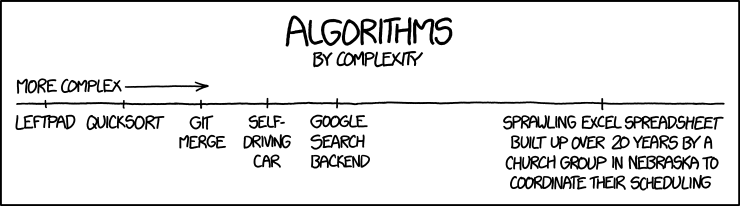
\includegraphics[width =
0.8\textwidth]{figures/algorithms.png} \caption{An \textit{xkcd} cartoon
captures the ballooning complexity and lack of transparency that can result from
many people using a spreadsheet with embedded macros. This practice can be a
critical barrier to reproducibility and transparency in biomedical research, yet
is still a common practice in many biomedical laboratories. \textit{Source: xkcd
by Randall Munroe}} \label{fig:spreadsheet} \end{figure}

\textbf{Using a structured data format to record data.} Every extra step of data
formatting is another chance to introduce an error in the data. The format in which experimental data is recorded can have a large influence on how easy and likely it is to implement reproducibility tools in later stages of data pre-processing, analysis, and visualization. One key concept for improving the reproducibility of experimental data collection is understanding how to create and use structured data formats, of which the ``tidy" data format is one popular implementation. 

Recording data in a ``structured" format brings many benefits for later stages of the research process, especially in terms of improving reproducibility. Therefore, by keeping research data pipelines simple---which can be more easily achieved if
data is initially recorded in a format amenable to later data pre-processing,
analysis, and visualization---researchers can decrease the potential for errors
in the data and therefore improve the rigor and reproducibility of their
research. Data that is in a structured tabular, two-dimensional format is vastly easier for collaborators like statisticians to understand and work with, without additional data formatting \cite{broman2018data}; however, many biomedical researchers are unaware of this simple yet powerful strategy in data recording and how it can improve the efficiency and effectiveness of collaborations \cite{ellis2018share}. ``When a researcher turns over a properly tidied dataset, it dramatically decreases the workload on the statistician and minimizes the likelihood of errors during analysis. By taking the time to tidy the data, the data generator, who knows the details of the data generated better than anyone else, can expect to get the analysis back sooner and can be more confident in its accuracy." \cite{ellis2018share}

The ``tidy" data format is one implementation of a structured data format that has quickly gained popularity among statisticians and data scientists since it was defined in a 2014 paper \cite{wickham2014tidy}. The ``tidy" data
format plugs into the \textit{tidyverse} framework, which enables powerful and
user-friendly data management, processing, and analysis by combining simple
tools to solve complex, multi-step problems, and this framework is enabled by
ensuring those simple tools share a common interface: a ``tidy" data format
\cite{ross2017declutter, silge2016tidytext, wickham2016ggplot2, wickham2016r}. Since the \textit{tidyverse} tools are simple and share a
common interface, they are easier to learn, use, and combine than tools created
in the classical R framework \cite{ross2017declutter, lowndes2017our,
reviewer2017review, mcnamara2016state}. This \textit{tidyverse} framework is
quickly becoming the standard taught in introductory R courses and books
\cite{hicks2017guide, baumer2015data, kaplan2017teaching, stander2017enthusing,
reviewer2017review, mcnamara2016state}, ensuring ample training resources for
researchers new to programming, including books (e.g., \cite{baumer2017modern,
lifesciencesR}, some freely available online, e.g., \cite{wickham2016r}),
massive open online courses (MOOCs), onsite university courses
\cite{baumer2015data, kaplan2017teaching, stander2017enthusing}, and Software
Carpentry workshops \cite{wilson2014software, pawlik2017developing}. Further,
tools that extend the tidyverse have been created to enable high-quality data
analysis and visualization in several domains, including text mining
\cite{silge2017text}, microbiome studies \cite{mcmurdie2013phyloseq}, natural
language processing \cite{RJ-2017-035}, network analysis \cite{RJ-2017-023},
ecology \cite{hsieh2016inext}, and genomics \cite{yin2012ggbio}. Further, by using a consistent structured format like the ``tidy" format across many or all data in a research project, it becomes much easier to create solid, well-tested code scripts for data pre-processing and analysis and to apply those scripts consistently and reproducibly across the datasets from multiple experiments \cite{broman2018data}.

This topic will
be covered in a \textit{Principles} module on ``Principles and power of
structured data formats", two \textit{Implementation} modules on ``The 'tidy'
data format: an implementation of a structured data format" and ``Designing
templates for tidy data collection", and one \textit{Example} module called
``Example: Creating a template for 'tidy' data collection". Key readings for this section will be \cite{broman2018data} and \cite{wickham2014tidy}. 

\textbf{Managing all research project files in a single, structured directory.}
Reproducbility can also be improved, starting at the data recording stage or
earlier, by using single, structured directory to store all files related to the
project. This ``project" framework has recently been encouraged by a number of
researchers as a way to enable computationally reproducible research, especially
for research conducted by teams \cite{marwick2018packaging,
parker2017opinionated, lowndes2017our}. Some have suggested that if researchers learn better practices for cleanly and consistently managing project files, it will help increase they willingness to share those files and so meet standards of reproducibility \cite{marwick2018packaging}. This practice can also improve the efficiency and effectiveness of collaborations with statisticians, as it allows the researchers to share critical research project files---raw data, pre-processed data, and code scripts for extracting the pre-processed data from the raw data \cite{ellis2018share, shade2015computing}---in a single, zipped file. If a consistent structure is used for these directories across different research projects, it can substantially increase the efficiency of, and reduce errors in, data pre-processing and analysis, as code scripts can be created that can be re-used across different project directories with few required changes \cite{marwick2018packaging}.

One implementation of this is as an RStudio ``Project". In RStudio, a research can collect all research project files in a single, structured directory and save this directory of a ``Project" \cite{rstudiousingprojects}. When the researcher opens this ``Project", RStudio is open with the working directory set to the top level of the project directory, encouraging the use of transportable relative pathnames in code that reads in and writes out data and other files from the R code. RStudio ``Projects" allow easy integration with version control tools (\textit{git}) and online platforms for sharing a directory under version control (\textit{GitHub}, \textit{GitLab}). In particular, ``Projects" in RStudio can interface directly (with buttons) with GitHub. 

RStudio allows users to create their own
custom ``Project" template, suited to a specific type of data analysis or
software development, which can then be registered and accessed by other users
\cite{rstudioprojecttemplate}. While a ``Project" can have any internal
structure, a common structure can be enforced for a certain type of project
through the creation of a new ``Project" template, which defines the required
subdirectories, structure, and file names of common elements that must exist in
the project \cite{rstudioprojecttemplate}. If there is a standard for organizing files for a researcher's scientific area, this format can be encoded as a reusable template; use of the structure imposed by this template will make it easier for other researchers in the field to easily navigate code and data that is made public in efforts to increase reproducibility \cite{marwick2018packaging}. This template, when selected from a menu bar  in RStudio by a
future user, will create a new directory with a ``skeleton" structure,
potentially including templated files (e.g., for metadata) \cite{rstudioprojecttemplate}.

This topic will be
covered in a \textit{Principles} module on the ``Power of using a single
structured 'Project' directory for storing and tracking research project files",
an \textit{Implementation} module on ``Creating 'Project' templates", and an
\textit{Example} module called ``Example: Creating a 'Project' template".

\textbf{Implementing version control.} As a research project progresses, a typical practice in many experimental research groups is to save new versions of files (e.g., 'draft1.doc', 'draft2.doc') \cite{bryan2018excuse}, so that changes can be reverted. However, this practice leads to an explosion of files, and it becomes hard to track which files represent the ``current" state of a project. Version control---which tracks and documents changes to any documents that the user chooses to track in a directory---allows researchers to edit and change research project files more cleanly, keeping a single copy of each file in the directory rather than multiple versions, while maintaining the power to backtrack to previous versions. Further, with version control, ``commit messages" must be included to explain any changes, making both the changes and the reasoning behind them transparent. 

Once a researcher has learned to use git on their own computer for local version control, they can begin using version control 
platforms (e.g., GitLab, GitHub) to collaborate with others in their research
group while keeping the project under version control \cite{bryan2018excuse, shade2015computing}. Projects saved in a single, structured directory
can be easily put under \textit{Git} version control in \textit{RStudio}, which
includes a pane that allows users to work under version control without learning
command-line version control language and, if desired, easily connect the
project with an online version of the project hosted on \textit{GitHub}. These platforms allow
the all collaborators to share a current version of a project directory 
(similar to Dropbox), but in a way that allows easy use of version control 
and that is more efficient for exploring (and, when necessary, undoing) the changes 
each team member has made to project files \cite{bryan2018excuse}. 

The use of \textit{Git} has been encouraged as a tool to enable reproducible research \cite{piccolo2016tools, ram2013git, bryan2018excuse, lowndes2017our, cetinkaya2017infrastructure}. However, for many years, use of version control required use of the command line,
limiting its accessibility to researchers with limited programming experience.
However, graphical interfaces have removed this barrier, and RStudio has 
particularly user-friendly tools for implementing version control. At CSU, we have found that Git and GitHub can be taught fairly quickly to researchers in their first programming course, so that they can successfully use GitHub to submit class assignments when taught through the RStudio / GitHub interfaces; others have had similar success at other institution \cite{bryan2018excuse}.

This
topic will be covered in two \textit{Principles} modules called ``Harnessing
version control for transparent data recording" and ``Enhance the
reproducibility of collaborative research with version control platforms" as
well as an \textit{Implementation} module on ``Using git and GitLab to implement
version control". A key supplemental reading in this section will be \cite{bryan2018excuse}.

\underline{\textbf{Improving the Reproducibility of Experimental Data
Pre-Processing}}

The second sequence will provide principles and tools for increasing the
computational reproducibility at an early stage of biomedical research, as
experimental data is pre-processed. By ``pre-processing", we mean the steps 
taken to convert data from the raw data either collected by hand or output
by equipment into a format ready for steps in data analysis. We will focus
particularly on improving the reproducibility of this step for complex 
raw data output by research equipment, for example: feature identification 
and quantification in mass spectrometry data, gating in flow cytometry data, 
image pre-processing for functional magnetic resonance imaging (fMRI), as well
as general pre-processing steps like normalization and scaling. This sequence will include nine modules covering three main topics: 

\textbf{Using code scripts to pre-process experimental data.} The experimental data collected for biomedical research often requires 
pre-processing before it can be analyzed (e.g., gating of flow cytometry data, 
peak finding and quantification for LC / MS metabolomics data). 

While 
often proprietary point-and-click software is available for this pre-processing,
use of such software can limit the transparency and reproducibility of this 
pre-processing stage of the analysis and is 
time-consuming for repeated tasks over large research projects. Scriptable
software tools bring key advantages compared to GUI software in terms of data
pre-processing, including that open-source choices are transparent and often are more robust and easier to extend \cite{cetinkaya2017infrastructure, huber2015orchestrating,
preeyanon2014reproducible, piccolo2016tools, baumer2017lessons}. While many of the pre-processing tasks required for biomedical experimental data are complex (e.g., feature identification and quantification, gating), R has many free, open-source package extensions that can complete these tasks, many hosted on Bioconductor \cite{huber2015orchestrating}.

Using a code script for pre-processing is also critical for fostering effective and efficient collaborations with statisticians. Point-and-click software is used interactively and often does not create a history of steps and choices, at least not in a format that is easy for a statistician to navigate, understand, and check \cite{peng2011reproducible, pernet2015improving}. Statisticians have clearly stated that, to ensure research is reproducible and that a collaboration is efficient, they would like to receive raw experimental data (e.g., the direct output from experimental equipment), the processed data (preferably in a 'tidy' format), and an ``explicit and exact recipe" for how the processed data was derived from the raw data \cite{ellis2018share}. An R script provides this ``explicit and exact recipe" describing how the raw data was pre-processed. Scripted pre-processing can also help reduce the temptation to manually edit data, including manually changing file formats, during pre-processing, which prevents reproducibility and impedes transparency \cite{pernet2015improving}.

When a code script is used for pre-processing experimental data, it can also improve the efficiency of pre-processing, as scripts can often be re-used with minimal changes for data from new experiments \cite{pernet2015improving}. For example, it can take [amount of time] to manually gate the experimental data output from a flow cytometer, and this process must be repeated with each new experiment. By comparison, writing an R script for automated gating of the data may take more time for the first experiment, but then can process data from further experiments at a fraction of the time. While laboratory-based researchers must invest time to learn some programming to be able to use scripts for pre-processing, this time investment is rewarded by a substantial improvement of the efficiency of future pre-processing tasks. 

However, it is critical to provide some
training on the use of these tools, and how they can improve transparency and reproducibility, for researchers new to programming. Expertise
with a scripting language is not universal across the biomedical community,
although literacy in programming is increasing in the sciences
\cite{ram2013git}, and many now recommend programming as a critical skill for
all biology Ph.D. students \cite{list2017ten}. 

This topic will be covered in one
\textit{Principles} module on ``Principles and benefits of scripted
pre-processing of experimental data" and two \textit{Implementation} modules
called ``Introduction to scripted data pre-processing in R" and ``Simplify
scripted pre-processing through R's 'tidyverse' tools".

\textbf{Working with complex data types during pre-processing.} Many key R functions output data in a form that is 'untidy' \cite{robinson2014broom}. This is particularly true for raw data from many biomedical experiments, especially machine-generated data (e.g., output from flow cytometer or mass spectrometer). Raw data from many biomedical experiments, especially those that
use high-throughput techniques, can be very large and complex. Because of the 
scale and complexity of these data, software for pre-processing the data in R
often uses complex, 'untidy' data formats. Biocondutor, which hosts many R packages useful for preprocessing and analyzing experimental biomedical data, relies heavily on an object-oriented framework, with functions outputting data in object formats S4 object formats, aiding interoperability among Bioconductor packages and helping to keep together different types of data from an experiment (e.g., for microarray experiments, array-based expression measurements kept together with phenotype and administrative data from the experiment) throughout the code \cite{gentleman2004bioconductor}. These S4 objects are 'untidy', in the sense that they do not follow the format required for 'tidyverse' R tools \cite{biobroom}

While these formats are well-justified within open-source software for pre-processing complex biomedical data, they add a critical barrier for researchers wishing
to implement reproduciblity tools, especially tools from the popular and user-friendly 'tidyverse' collection of R package externsions \cite{robinson2014broom}. While this hurdle can be surmounted by skilled R programmers, it creates a barrier for researchers who are learning scripting tools \cite{robinson2014broom}, and it can reduce transparency of analysis by requiring obscure, lengthy code to extract and tidy data from the complex data object \cite{robinson2014broom}. Very recently, the \textit{broom} and \textit{biobroom} R packages have been developed 
to extract a 'tidy' dataset from many common complex data formats that are output by R functions, including much of the output formats common for preprocessing biomedical experimental data \cite{robinson2014broom, biobroom}.
These tools create a clean, simple connection between the complex data formats
often used in pre-processing experimental data and the 'tidy' format
required to use the 'tidyverse' tools now taught in many introductory R courses, making it more straightforward for a researcher new to R programming develop a scripted R workflow from data preprocessing through to data analysis and visualization using 'tidyverse' tools. The \textit{biobroom} package, in particular, can 'tidy' data within many popular Bioconductor data formats, including \textit{ExpressionSet} objects \cite{biobroom}.

This topic will be covered in a \textit{Principles} module on ``Complex data types in
experimental data pre-processing", a \textit{Implementation} module on ``Complex
data types in R and Bioconductor", and an \textit{Example} module called
``Example: Converting from complex to 'tidy' data formats".

\textbf{Reproducible data pre-processing protocols.} ``Experimental protocols in molecular biology are fully published lists of ingredients and algorithms for creating specific substances or processes. Accuracy of an experimental claim can be checked by complete obedience to the protocol. This standard should be adopted for algorithmic work in [computational biology and bioinformatics]. Portable source code should accompany each published analysis, coupled with the data on which the analysis is based." \cite{gentleman2004bioconductor}

Reproducibility tools can be used to create reproducible data pre-precessing protocols---documents that combine code and text in a ``knitted" document, which can be re-used to ensure data pre-processing is consistent and reproducible across research projects. The R extension package RMarkdown can be used to create documents that combine code and text in a 
``knitted" document, and it has become a popular tool 
for improving the computational reproducibility and 
efficiency of the data analysis stage of research. This tool can also be used earlier in the research process, however, to improve reproducibility of pre-processing steps. 

Pre-processing software allows many parameter choices, which can lead to an explosion of possible combinations of parameter choices in pre-processing data \cite{munafo2017manifesto, shade2015computing, pernet2015improving}. To ensure transparent and high-quality biomedical research, it is important to be thoughtful in selecting the parameter values, and to keep a detailed record of which parameter values were selected and why throughout pre-processing. This helps make it easier and clearer to share the pre-processing ``recipe" with collaborators and as part of publishing a journal article that meets reproducibility guidelines. It also helps ensure a continuity of methods across a research group, where a research laboratory can be sure the same pre-processing is maintained as researchers join and leave the group \cite{shade2015computing}.

This topic will be covered in a \textit{Principles} module called ``Introduction to reproducible data pre-processing protocols", an \textit{Implementation} module on ``RMarkdown
for creating reproducible data pre-processing protocols", and an
\textit{Example} module called ``Example: Creating a reproducible data
pre-processing protocol". 

\underline{\textbf{Choice of tools to include in ``Implementation" modules.}}

To improve reproducibility practices among our target audience, it is important
that we provide them with some instruction on how to implement the
reproduciblity principles we cover. For some of these principles, there are
several reasonable and well-developed tools that could be used for
implementations. However, few researchers are interested in learning every tool,
and instead would prefer to learn one set of tools that ``just work", and presenting a single set of tools improves the chance of trainees mastering the tools \cite{brown2018ten}.

We have chosen for the implementation portion of these
modules to focus on tools from the open-source R programming language. R can be
freely, quickly, and easily downloaded and installed to a user's computer,
allowing new users to get started quickly, a critical consideration for usable
scientific software \cite{list2017ten}. R has been maintained for over a decade
by the R Development Core Team and works with all major computing platforms,
ensuring  widespread access, stability, and compatability, also critical for
ease-of-use \cite{baumer2017lessons, altschul2013anatomy}. R offers a
well-developed environment for creating new tools that extend the core language
\cite{wickham2015r, gentleman2004bioconductor} and includes ample tools for documenting research workflows
\cite{xie2015dynamic, xie2016bookdown}. R's status as a common tool among statisticians and biostatisticians means that its use in early stages of
experimental data recording and pre-processing can help foster closer
collaborations between laboratory-based scientists and statisticians throughout
the research process. R can be scaled as the volume of data in projects grows
\cite{list2017ten}, as it includes tools to interface with distributed computing
platforms (e.g., \textit{Hadoop} \cite{pathak2014rhadoop}, \textit{Spark}
\cite{sparklyr}), and its scripts can be integrated within workflow management
systems (e.g., \textit{Galaxy} \cite{goecks2010galaxy, walker2016models}). Some
of the implementation tools---git and GitLab, for example---are separate from R
but can be mastered much more easily if trainees are taught to use them through
RStudio's user-friendly interfaces rather than using the command line or other
alternative interfaces. RStudio is a free, open-source Integrated Development Environment (IDE) for the R programming language. It is actively developed by a team of some of the best R programmers worldwide, including the developers of the ``tidyverse" (including the \textit{ggplot2} plotting system), the most popular tools for literate programming in R (\textit{knitr} and \textit{RMarkdown}) and the Shiny web application system. 

We have also selected to focus on this set of tools for
the \textit{Implementation} modules because two members of our team (Anderson
and Lyons) use R daily for their own research and so are able to provide much
better instruction and details on using this set of tools than alternative tools
for the same tasks. Dr. Anderson also regularly teaches students in her
department how to use this set of tools through a graduate-level course and has
developed techniques for helping students new to programming to master R using
the RStudio interface, including using RStudio's interface to use RMarkdown,
track a project under git version control, and connect to version control
platforms to improve collaborative work. 

We appreciate that many researchers do not know the R language, and
some of them may want to learn more about improving reproducibility without
needing to learn a new programming language. For this reason, we have
deliberately separated the ``Principles" and ``Examples" content in our modules
from the ``Implementation" modules, so that a researcher can select a track of
our modules that does not require programming knowledge. Further, while all of
the ``Implementation" modules are conceptually focused on tools that an R
programmer would use, several of the modules could be appreciated and used to
improve reproducibility without a mastery of R. For example, RStudio and its
``Projects" functionality can be used to help manage research project files,
keep them under version control, and interface with GitLab to work
collaboratively without using any R code within the project. Similarly, while
the ``tidy" data format is currently an important implementation common within R
for structuring data, understanding its principals and characteristics does not
require any knowledge of R. In our table of example ``tracks" that a trainee
could follow, the track for an example Principal Investigator gives one example
of a track that would not require any prior knowledge of R or other programming
languages.   


\begin{landscape}\begingroup\fontsize{9}{11}\selectfont
\rowcolors{2}{white}{gray!6}

\begin{longtable}[t]{>{\bfseries\raggedright\arraybackslash}p{10em}>{\raggedright\arraybackslash}p{30em}>{\raggedright\arraybackslash}p{15em}>{\raggedright\arraybackslash}p{3em}>{\raggedright\arraybackslash}p{15em}}
\caption{\label{tab:}Modules for the first sequence, \textbf{'Improving the Reproducibility of Experimental Data Recording'}. The color of each module's title indicates whether the module focuses on \textbf{Principles} (blue), \textbf{Implementation} (red), or \textbf{Case study examples} (black). This table is continued over several pages.}\\
\hiderowcolors
\toprule
Module title & Description of module content & Objectives (After taking the module, the trainee can ...) & Video length & Extra educational materials\\
\midrule
\endfirsthead
\caption[]{Modules for the first sequence, \textbf{'Improving the Reproducibility of Experimental Data Recording'}. The color of each module's title indicates whether the module focuses on \textbf{Principles} (blue), \textbf{Implementation} (red), or \textbf{Case study examples} (black). This table is continued over several pages. \textit{(continued)}}\\
\toprule
Module title & Description of module content & Objectives (After taking the module, the trainee can ...) & Video length & Extra educational materials\\
\midrule
\endhead
\
\endfoot
\bottomrule
\endlastfoot
\showrowcolors
\textcolor{blue}{\textbf{Separating data recording and analysis}} & Many biomedical laboratories currently use spreadsheets, with embedded macros, 
      to both record and analyze experimental data. This practice empedes the transparency
      and reproducibility of both data recording and data analysis. In this module, we 
      will describe this common practice and explain how it impedes the transparency and
      reproducibility of data recording and analysis. We will then outline alternative
      approaches that separate the steps of data recording and data analysis and explain
      how these alternative approaches can improve the reproducbility of biomedical 
      research. & \tabitem Explain the difference between data recording and data analysis 

     \tabitem Understand why collecting data on spreadsheets with embedded macros
        impedes transparency and reproducibility 

      \tabitem List alternative approaches that separate data recording and data analysis to 
        improve transparency and reproducibility & 15 & \tabitem Discussion questions about data recording approaches the trainee has 
      previously used in research projects and the benefits
      and limitations of those approaches in terms of data transparency and 
      reproducibility 

    \tabitem Short audio recording of two Co-Is giving their
      own answers to these discussion questions\\
\textcolor{blue}{\textbf{Principles and power of structured data formats}} & The format in which experimental data is recorded can have a large influence
      on how easy and likely it is to implement reproducibility tools in later stages of
      data pre-processing, analysis, and visualization. Recording data in a 'structured'
      format brings many benefits for later stages of the research process, 
      especially in terms of improving reproducibility.
      In this module, we will explain what makes a dataset 'structured' and
      why this format is a powerful tool for reproducible research. & \tabitem List the characteristics of a structured data format 

      \tabitem Describe how using a structured data format when recording experimental 
      data can improve the transparency and reproducibility of research

      \tabitem Outline other benefits of using a structured format when recording data & 10 & \tabitem Applied exercise: For example datasets, specify whether each is in a 
      structured data format and, in cases where it is not, draft a structured
      format that could be used to record the data 

    \tabitem Video walking trainees 
      through solutions to the applied exercise\\
\textcolor{red}{\textbf{The 'tidy' data format: an implementation of a structured data format}} & The 'tidy' data format is one implementation of a structured data format that
  was introduced in a 2014 paper and has since quickly 
  gained popularity among statisticians and data scientists. By consistently 
  using this data format, researchers have found they can employ combinations 
  of simple, generalizable tools to perform complex tasks in data processing, 
  analysis, and visualization. In this module, we will explain what characteristics determine
  if a dataset is 'tidy' and how use of the 'tidy' implementation of a structure 
  data format can improve the ease and efficiency
  of 'Team Science', including collaborations with statisticians. & \tabitem List characteristics defining the  
    the 'tidy' structured data format 

  \tabitem Explain the difference between the ideas of a structured data format (general 
    concept) and the 'tidy' data format (one implementation of that general format
    that is now particularly popular in data analysis) & 15 & \tabitem Quiz questions: For example datasets, correctly identify which of the 'tidy'
  data principles the dataset has or lacks 

  \tabitem Video giving answers and explanations
  for quiz questions, including showing 'tidy' versions of each example dataset 

  \tabitem Link to paper that established the 'tidy' data format\\
\textcolor{red}{\textbf{Designing templates for tidy data collection}} & This module will move from the principles of the 'tidy' data format to the 
      practical details of designing a 'tidy' data format to use when collecting 
      experimental data. We will describe common issues that prevent many real datasets from
      experimental research projects from being 'tidy' and show how these issues
      can be avoided when deciding the format in which to record experimental data.
      We will also provide rubrics and a checklist to help determine if a 
      data collection template complies with a 'tidy' format. & \tabitem Identify characteristics that keep a dataset from being 'tidy'
      
      \tabitem Convert data from an 'untidy' to a 'tidy' format & 20 & \tabitem Applied exercise: For an 'untidy' dataset, identify what 
      characteristics keep it from being 'tidy', and convert design a 'tidy' format

  \tabitem Video providing a detailed solution to the applied exercise\\
\textcolor{black}{\textbf{Example: Creating a template for 'tidy' data collection}} & In this module, we will walk through an example of creating a template to collect
      data in a 'tidy' format for a laboratory-based research project. As an example,
      we will use a research project headed by one of our Co-Is on drug efficacy in 
      murine tuberculosis models. We will walk through the 'untidy' format 
      initially used to collect data for this project, explain how this format 
      differed from a 'tidy' format, and show how we changed the format to be 'tidy'.
      Finally, we will show examples of how the experimental data can easily be 
      cleaned, analyzed, and visualized using reproducible tools once it is in a 
      'tidy' format. & \tabitem Understand how the principles of 'tidy' data can be applied 
      when recording experimental
      data for a real, complex research project;

      \tabitem List some advantages of using a 'tidy' data format for the example project & 15 & \tabitem Discussion questions, including listing examples of how experimental datasets
      the trainee has previously worked with or is currently working with are 'untidy' and
      how they could be converted to a 'tidy' format 

    \tabitem Short audio recording of two Co-Is giving their
      own answers to these discussion questions\\
\addlinespace
\textcolor{blue}{\textbf{Power of using a single structured 'Project' directory for storing and tracking research project files}} & To improve the computational reproducibility of a research project, researchers
      can use a single 'Project' directory to collectively store 
      all research data (raw and pre-processed), meta-data, code for data pre-processing,
      and research products further along the research pipeline (e.g., paper drafts, 
      figures, code for data analysis). In this 
      module, we will explain how using this practice from the 
      start of a research project improves the reproducibility of the projects, as well
      as facilitates other tools to improve reproducibility,
      including version control. Finally, we will 
      list some of the common components and subdirectories to include
      in the structure of a 'Project' directory, including subdirectories for raw and
      pre-processed experimental data. & \tabitem Describe a 'Project' directory, including common components and subdirectories 

      \tabitem List how collecting all research data and other files related 
      to a research project in a single 'Project' directory
      improves the reproducibility of a research project 

      \tabitem Describe how experimental data collection can be integrated with a
      research 'Project' directory & 20 & \tabitem Quiz questions: Test the trainee's understanding of a structured
      'Project' directory, what common components it may include, and the benefits
      of structuring research project files 
      within a single 'Project' directory from the beginning of the
      research project 

      \tabitem Video with detailed answers and discussion of quiz questions\\
\textcolor{red}{\textbf{Creating 'Project' templates}} & Researchers can use RStudio's 'Projects' interface to implement the structured
      collection of files for a research project in a single directory, with the added
      benefits that this interface faciliates use of version control. 
      Researchers can gain even more benefits, in terms of improving both the reproducibility
      and efficiency of research, by using a consistent structure for the 'Project' 
      directories for all of the research projects for a research group. We will demonstrate 
      how to implement structured project directories through RStudio,
      as well as how RStudio enables the creation of a template for all of a 
      research group's 'Project' directories, so a new project can be initialized
      with a skeleton directory that follows a directory format established
      by the research group. & \tabitem Be able to create a structured `Project` directory within RStudio 
      to use to consistently and reproducibly manage all files for a research project

     \tabitem Understand how RStudio can be used to create a template
      to use to create consistently-structured research 'Project' directories & 25 & \tabitem Discussion questions, including descriptions of how the trainee has saved and
      tracked research project files for previous research projects and what barriers,
      if any, these practices introduced in terms of the reproducibility and efficiency
      of research 

    \tabitem Short audio recording of two Co-Is discussing their answers to these questions\\
\textcolor{black}{\textbf{Example: Creating a 'Project' template}} & In this module, we will walk through a real example, based on the experiences of
      one of our Co-Is, of establishing the format 
      for a research group's 'Project' template, creating that template using RStudio,
      and initializing a new research project directory using the created template.
      This example will be from a laboratory-based research group that studies the efficacy of 
      tuberculosis drugs in a murine model. & \tabitem Create a 'Project' template in RStudio to use to initialize 
      consistently-formatted 'Project' directories to store all files related to 
      a research project
  
      \tabitem Initialize a new 'Project' directory using this template & 15 & \tabitem Applied exercise: Create and save a 'Project' 
      template that meets specifications provided for an example research group; 

     \tabitem Video demonstrating a detailed solution 
      to the applied exercise.\\
\textcolor{blue}{\textbf{Harnessing version control for transparent data recording}} & As a research project progresses, a typical practice in many experimental 
      research groups is to save new versions of files (e.g., 'draft1.doc', 'draft2.doc'),
      so that changes can be reverted. However, this practice 
      leads to an explosion of files, and it becomes hard to track 
      which files represent the 'current' state of a project. Version control allows
      researchers to edit and change research project files more cleanly, while maintaining
      the power to 'backtrack' to previous versions. Further, with version control,
      messages can be included to explain any changes.
      In this module, we will explain what version
      control is and how it can be used in research projects to improve the transparency 
      and reproducibility of research, particularly for transparent data recording. & \tabitem Describe version control and what it does 

      \tabitem Explain how version control can be used to improve reproducibility at 
      the data recording stage of research & 10 & \tabitem Discussion questions, including discussion of how the trainee has 
      managed evolving research project files in previous projects and any barriers
      those practices introduced in conducting efficient and reproducible research 

      \tabitem Short audio recording of two Co-Is giving their
      own answers to these discussion questions\\
\textcolor{blue}{\textbf{Enhance the reproducibility of collaborative research with version control platforms}} & Once a researcher has learned to use git on their own 
      computer for local version control, they can begin using version control 
      platforms (e.g., GitLab, GitHub) to collaborate with others in their research
      group while keeping the project under version control. These platforms allow
      the all collaborators to share a current version of a project directory 
      (similar to Dropbox), but in a way that allows easy use of version control 
      and that is more efficient for exploring (and, when necessary, undoing) the changes 
      each team member has made to project files. In this module, we will describe 
      why a research team may want to use a version control platform like GitLab 
      to work collaboratively on a project. & \tabitem List the benefits of using a version control platform like GitLab, rather 
      than Dropbox, to share project files, 
      particularly in terms of improving transparency and reproducibility 

     \tabitem Describe the difference between version control (e.g., git) and 
      a version control platform (e.g., GitLab) & 10 & \tabitem Discussion questions: Describe how you have shared research project 
    files in past research projects---email? Dropbox? Department servers?

    \tabitem Short audio file with two Co-Is discussing their answers\\
\textcolor{red}{\textbf{Using git and GitLab to implement version control}} & For many years, use of version control required use of the command line,
  limiting its accessibility to researchers with limited programming experience.
  However, graphical interfaces have removed this barrier, and RStudio has 
  particularly user-friendly tools for implementing version control.
  In this module, we will show how to use 
  \textit{git} through RStudio's user-friendly interface and how to connect from a local
  computer to \textit{GitLab} through RStudio. & \tabitem Understand how to set up and use \textit{git} through RStudio's interface 

  \tabitem Understand how to connect with \textit{GitLab} through RStudio to collaborate on  
  research projects while maintaining version control & 20 & \tabitem Applied exercise: Use RStudio to 
  initialize \textit{git} version control for a directory 
  and to make several tracked changes. Create a matching \textit{GitLab} repository and use
  RStudio to push local changes to this GitLab version of the directory

  \tabitem Video 
  walking trainees through a detailed solution to the exercise\\*
\end{longtable}
\rowcolors{2}{white}{white}\endgroup{}
\end{landscape}



\begin{landscape}\begingroup\fontsize{10}{12}\selectfont
\rowcolors{2}{white}{gray!6}

\begin{longtable}[t]{>{\bfseries\raggedright\arraybackslash}p{10em}>{\raggedright\arraybackslash}p{28em}>{\raggedright\arraybackslash}p{14em}>{\raggedright\arraybackslash}p{3em}>{\raggedright\arraybackslash}p{14em}}
\caption{\label{tab:}\label{tab:content_two} Modules for the second sequence, \textbf{'Improving the Reproducibility of Experimental Data Pre-Processing'}. The color of each module's title indicates whether the module focuses on \textbf{Principles} (blue), \textbf{Implementation} (red), or \textbf{Case study examples} (black). This table is continued over several pages.}\\
\hiderowcolors
\toprule
Module title & Description of module content & Objectives (After taking the module, the trainee can ...) & Video length & Extra educational materials\\
\midrule
\endfirsthead
\caption[]{\label{tab:content_two} Modules for the second sequence, \textbf{'Improving the Reproducibility of Experimental Data Pre-Processing'}. The color of each module's title indicates whether the module focuses on \textbf{Principles} (blue), \textbf{Implementation} (red), or \textbf{Case study examples} (black). This table is continued over several pages. \textit{(continued)}}\\
\toprule
Module title & Description of module content & Objectives (After taking the module, the trainee can ...) & Video length & Extra educational materials\\
\midrule
\endhead
\
\endfoot
\bottomrule
\endlastfoot
\showrowcolors
\textcolor{blue}{\textbf{Principles and benefits of scripted pre-processing of experimental data}} & The experimental data collected for biomedical research often requires 
      pre-processing before it can be analyzed (e.g., gating of flow cytometry data, 
      peak finding and quantification for LC / MS metabolomics data). While 
      often proprietary point-and-click software is available for this pre-processing,
      use of such software can limit the transparency and reproducibility of this 
      pre-processing stage of the analysis and is 
      time-consuming for repeated tasks over large research projects.
      In this module, we will explain how scripted pre-processing, especially using open source software, 
      can improve the transparency, reproducibility, and
      transparency of research. & \tabitem Define 'pre-processing' of experimental data 

      \tabitem Describe how point-and-click software limits transparency and reproducibility
      of data pre-processing

      \tabitem Describe an open source
      code script and explain how it can enable pre-processing 
      experimental data & 15 & \tabitem Discussion questions, including common pre-processing needs and 
    practices in their research area
      
      \tabitem Short audio recording of two Co-Is giving their
      own answers to these discussion questions\\
\textcolor{red}{\textbf{Introduction to scripted data pre-processing in R}} & In this module, we will show how researchers can implement scripted pre-processing
    of experimental data through use of R scripts. 
    We will demonstrate the difference between interactive coding and the
      use of code scripts, using R for examples. We will then demonstrate how to 
      create, save, and run an R code script for a simple data cleaning task. & \tabitem Describe what an R code script is and how it differs from interactive
      coding in R 

      \tabitem Create and save an R script to perform a simple data 
      pre-processing task 
  
      \tabitem Run an R script

      \tabitem List some popular packages in R for 
      pre-processing biomedical data & 10 & \tabitem Applied exercise: Given a simple example dataset and a data cleaning task, 
      write and run an R script to perform the task. Then adapt that script to re-use
      it on a second dataset. Hints will be 
      provided for those new to R 

      \tabitem Video providing a detailed
      walk-through of a solution to the applied exercise\\
\textcolor{red}{\textbf{Simplify scripted pre-processing through R's 'tidyverse' tools}} & The R programming language now includes a collection of 'tidyverse' extension 
      packages that enable user-friendly yet powerful work with experimental data,
      including pre-processing and exploratory visualizations. The principle behind
      the 'tidyverse' is that a collection of simple, general tools can be joined 
      together to solve complex problems, as long as a consistent format is used 
      for the input and output of each tool (the 'tidy' data format taught in other
      modules). In this module, we will explain why this 'tidyverse' system is so
      powerful and how it can be leveraged within biomedical research, especially for
      reproducibly pre-processing experimental data. & \tabitem Define R's 'tidyverse' system 

      \tabitem Explain how the 'tidyverse' collection
      of packages can be both user-friendly and powerful in solving many complex
      tasks with data 

      \tabitem Describe the difference between base R and
      R's 'tidyverse'. & 15 & \tabitem Quiz questions: What is R's 
      'tidyverse' is and why is it a powerful yet user-friendly tool for improving
      the reproducibility of research projects 

      \tabitem Video with detailed answers and explanations for the quiz questions 

      \tabitem Links to free sources for developing more 'tidyverse' coding 
        skills\\
\textcolor{blue}{\textbf{Complex data types in experimental data pre-processing}} & Raw data from many biomedical experiments, especially those that
  use high-throughput techniques, can be very large and complex. Because of the 
  scale and complexity of these data, software for pre-processing the data in R
  often uses complex, 'untidy' data formats. While these formats are necessary
  for computational efficiency, they add a critical barrier for researchers wishing
  to implement reproducibility tools. In this module, we will 
  explain why use of complex data formats is
  often necessary within open source pre-processing software 
  and outline the hurdles created in 
  reproducibility tool use among laboratory-based scientists. & \tabitem Explain why R software for pre-processing biomedical data often stores 
  data in complex, 'untidy' formats; 
  
  \tabitem Describe how these complex data formats can create barriers to 
  laboratory-based researchers seeking to use reproducibility tools for 
  data pre-processing. & 15 & \tabitem Quiz questions: Why are complex data formats
  often used within steps of experimental data pre-processing in open-source
  software and how does their use complicate the use of reproducibility tools
  
  \tabitem Video providing detailed
  answers to quiz questions\\
\textcolor{red}{\textbf{Complex data types in R and Bioconductor}} & Many R extension packages for pre-processing experimental data use complex (rather than
    'tidy') data formats within their code, and many output data in complex formats. 
    Very recently, the \textit{broom} and \textit{biobroom} R packages
  have been developed 
  to extract a 'tidy' dataset from a complex data format.
  These tools create a clean, simple connection between the complex data formats
  often used in pre-processing experimental data and the 'tidy' format
  required to use the 'tidyverse' tools now taught in many introductory R courses. In this module, we will describe the 'list' data structure,
    the common backbone for complex data structures in R, and well as provide tips on how to
  explore and extract data stored in R in this format, including through the 
     \textit{broom} and \textit{biobroom} packages. & \tabitem Describe the structure of R's 'list' data
      format 

      \tabitem Take basic steps to explore
      and extract data stored in R's complex, list-based structures
  
      \tabitem Describe what the \textit{broom} and \textit{biobroom} R packages can do 

      \tabitem Explain how converting data to a 'tidy' format can improve reproducibility & 15 & \tabitem Applied exercise: Starting with example data in a complex, list-based format, 
  explore the data and extract specified elements, including with the \textit{broom} and
  \textit{biobroom} packages; 
  
  \tabitem Video providing a detailed
  walk-through of the solution to this exercise\\
\addlinespace
\textcolor{black}{\textbf{Example: Converting from complex to 'tidy' data formats}} & We will provide a detailed example of a case where data pre-processing in R
      results in a complex, 'untidy' data format. We will
      walk through an example of applying automated gating to flow cytometry data. 
      We will demonstrate the complex initial format of this pre-processed data and then
      show trainees how a 'tidy' dataset can be extracted and used for further data
      analysis and visualization using the popular R 'tidyverse' tools. 
      This example will use real experimental data from on of our Co-Is 
      research on the immunology of tuberculosis. & \tabitem Describe how tools like \textit{biobroom} were used in this real 
    research example to convert from the complex data format from pre-processing to
    a format better for further data analysis and visualization

      \tabitem Understand how these tools would fit in 
      their own research pipelines & 20 & \tabitem Applied exercise: With an example dataset in a complex, 
      'untidy' data format in R, convert it to 
      a 'tidy' format and create simple plots with
      this 'tidy' dataset 

      \tabitem Video demonstrating a detailed solution to the applied
      exercise\\
\textcolor{blue}{\textbf{Introduction to reproducible data pre-processing protocols}} & Reproducibility tools can be used to create reproducible data pre-processing 
    protocols---documents that combine code and text in a 
  'knitted' document, which can be re-used to ensure data pre-processing is consistent
  and reproducible across research 
  projects. In this module, we will describe how
  reproducible data pre-processing protocols 
  can improve reproducibility 
  of pre-processing experimental data, as well as to ensure transparency, consistency,
  and reproducibility across the research projects conducted by a research team. & \tabitem Define a 'reproducible data pre-processing protocol' 
  
  \tabitem Explain how such protocols improve
    reproducibility at the data pre-processing phase 
  
  \tabitem List other benefits,
    including improving efficiency and consistency of data pre-processing & 15 & \tabitem Discussion questions: How reproducible data pre-processing 
  protocols can make biomedical research more reproducible at the data 
  pre-processing stage in the trainee's research area
  
  \tabitem Short audio 
  recording of two Co-Is giving their
  own answers to these discussion questions\\
\textcolor{red}{\textbf{RMarkdown for creating reproducible data pre-processing protocols}} & The R extension package RMarkdown can be used to create documents that combine code and text in a 
      'knitted' document, and it has become a popular tool 
      for improving the computational reproducibility and 
      efficiency of the data analysis stage of research. This tool can also be used earlier in the 
      research process, however, to improve reproducibility of pre-processing steps.
      In this module, we will provide detailed instructions on how to use RMarkdown
      in RStudio to create documents that combine code and text. We will show how an 
    RMarkdown document describing a data 
    pre-processing protocol can be used to efficiently apply the same data
    pre-processing steps to different sets of raw data. & \tabitem Define RMarkdown and the documents it can create 

      \tabitem Explain how RMarkdown can be used to improve the reproducibility
      of research projects at the data pre-processing phase 
  
      \tabitem Create a document in RStudio using 
      RMarkdown 
  
  \tabitem Apply it to several different datasets
  with the same format & 15 & \tabitem Applied exercise: Create, save, and render 
    their own RMarkdown document through RStudio 
  
  \tabitem Video providing a detailed
  walk-through of a solution to the applied exercise\\
\textcolor{black}{\textbf{Example: Creating a reproducible data pre-processing protocol}} & We will walk through an example of creating a reproducible protocol for the automated
      gating of flow cytometry data for a project on the immunology of tuberculosis
      lead by one of our Co-Is. This data pre-processing protocol was created 
      using RMarkdown and allows the efficient, transparent, and reproducible 
      gating of flow cytometry data for all experiments in the research group. We will
      walk the trainees through how we developed the protocol initially, 
      the final pre-processing protocol, how we apply this
      protocol to new experimental data. & \tabitem Explain how a reproducible data pre-processing protocol can be integrated
      into a real research project 

      \tabitem Understand how to design and implement a data
      pre-processing protocol to replace manual or point-and-click data pre-processing
      tools & 20 & \tabitem Quiz questions: Test understand of how and why we 
      created a reproducible data pre-processing protocols for this 
      pre-processing step, and how this improves reproducibility for the research group; 

      \tabitem Short video with a detailed discussion of quiz questions\\*
\end{longtable}
\rowcolors{2}{white}{white}\endgroup{}
\end{landscape}



\begin{landscape}\begin{table}[!h]

\caption{\label{tab:}Examples of how different types of trainees might use subsets of the training modules to meet their specific training needs.}
\centering
\fontsize{9}{11}\selectfont
\begin{tabular}[t]{>{\centering\arraybackslash}p{28em}ccccc}
\toprule
\multicolumn{1}{c}{} & \multicolumn{1}{c}{\makecell[c]{\textbf{Graduate student}\\who would like to\\learn in detail\\how to use\\reproducibility tools\\for data recording\\and pre-processing\\and is willing to learn\\R programming tools}} & \multicolumn{1}{c}{\makecell[c]{\textbf{Principal investigator}\\who does not program\\but would like to\\learn how his/her\\research team could\\improve reproducibility\\of data recording\\and pre-processing}} & \multicolumn{1}{c}{\makecell[c]{\textbf{Biostatistician}\\who would\\like to understand\\barriers faced by\\collaborators\\in implementing\\reproducibility\\principles early\\in research projects}} & \multicolumn{1}{c}{\makecell[c]{\textbf{Technician}\\in charge of\\running and\\pre-processing\\mass\\spectrometry\\data}} & \multicolumn{1}{c}{\makecell[c]{\textbf{Undergraduate}\\\textbf{student}\\who wants an\\introduction\\to improving\\reproducibility\\of data\\recording}}\\
\midrule
\addlinespace[0.3em]
\multicolumn{6}{l}{\textbf{Improving the Reproducibility of Experimental Data Recording}}\\
\hspace{1em}\tabitem Separating data recording and analysis & \cellcolor{pink}{Yes} & \cellcolor{pink}{Yes} & \cellcolor{pink}{Yes} & \cellcolor{white}{No} & \cellcolor{pink}{Yes}\\
\hspace{1em}\tabitem Principles and power of structured data formats & \cellcolor{pink}{Yes} & \cellcolor{pink}{Yes} & \cellcolor{white}{No} & \cellcolor{white}{No} & \cellcolor{pink}{Yes}\\
\hspace{1em}\tabitem The 'tidy' data format: an implementation of a structured data format & \cellcolor{pink}{Yes} & \cellcolor{pink}{Yes} & \cellcolor{white}{No} & \cellcolor{white}{No} & \cellcolor{white}{No}\\
\hspace{1em}\tabitem Designing templates for 'tidy' data collection & \cellcolor{pink}{Yes} & \cellcolor{pink}{Yes} & \cellcolor{white}{No} & \cellcolor{white}{No} & \cellcolor{white}{No}\\
\hspace{1em}\tabitem Example: Creating a template for 'tidy' data collection & \cellcolor{pink}{Yes} & \cellcolor{pink}{Yes} & \cellcolor{pink}{Yes} & \cellcolor{white}{No} & \cellcolor{white}{No}\\
\hspace{1em}\tabitem Power of using a single structured 'Project' directory for storing and tracking research project files & \cellcolor{pink}{Yes} & \cellcolor{pink}{Yes} & \cellcolor{white}{No} & \cellcolor{white}{No} & \cellcolor{pink}{Yes}\\
\hspace{1em}\tabitem Creating 'Project' templates & \cellcolor{pink}{Yes} & \cellcolor{white}{No} & \cellcolor{white}{No} & \cellcolor{white}{No} & \cellcolor{white}{No}\\
\hspace{1em}\tabitem Example: Creating a 'Project' template & \cellcolor{pink}{Yes} & \cellcolor{pink}{Yes} & \cellcolor{pink}{Yes} & \cellcolor{white}{No} & \cellcolor{white}{No}\\
\hspace{1em}\tabitem Harnessing version control for transparent data recording & \cellcolor{pink}{Yes} & \cellcolor{pink}{Yes} & \cellcolor{white}{No} & \cellcolor{white}{No} & \cellcolor{pink}{Yes}\\
\hspace{1em}\tabitem Enhance the reproducibility of collaborative research with version control platforms & \cellcolor{pink}{Yes} & \cellcolor{pink}{Yes} & \cellcolor{white}{No} & \cellcolor{white}{No} & \cellcolor{pink}{Yes}\\
\hspace{1em}\tabitem Using git and GitLab to implement version control & \cellcolor{pink}{Yes} & \cellcolor{white}{No} & \cellcolor{white}{No} & \cellcolor{white}{No} & \cellcolor{white}{No}\\
\addlinespace[0.3em]
\multicolumn{6}{l}{\textbf{Improving the Reproducibility of Experimental Data Pre-Processing}}\\
\hspace{1em}\tabitem Principles and benefits of scripted pre-processing of experimental data & \cellcolor{pink}{Yes} & \cellcolor{pink}{Yes} & \cellcolor{white}{No} & \cellcolor{pink}{Yes} & \cellcolor{white}{No}\\
\hspace{1em}\tabitem Introduction to scripted data pre-processing in R & \cellcolor{pink}{Yes} & \cellcolor{white}{No} & \cellcolor{white}{No} & \cellcolor{pink}{Yes} & \cellcolor{white}{No}\\
\hspace{1em}\tabitem Simplify scripted pre-processing through R's 'tidyverse' tools & \cellcolor{pink}{Yes} & \cellcolor{white}{No} & \cellcolor{white}{No} & \cellcolor{pink}{Yes} & \cellcolor{white}{No}\\
\hspace{1em}\tabitem Complex data types in experimental data pre-processing & \cellcolor{pink}{Yes} & \cellcolor{pink}{Yes} & \cellcolor{pink}{Yes} & \cellcolor{pink}{Yes} & \cellcolor{white}{No}\\
\hspace{1em}\tabitem Complex data types in R and Bioconductor & \cellcolor{pink}{Yes} & \cellcolor{white}{No} & \cellcolor{pink}{Yes} & \cellcolor{pink}{Yes} & \cellcolor{white}{No}\\
\hspace{1em}\tabitem Example: Converting from complex to 'tidy' data formats & \cellcolor{pink}{Yes} & \cellcolor{pink}{Yes} & \cellcolor{pink}{Yes} & \cellcolor{pink}{Yes} & \cellcolor{white}{No}\\
\hspace{1em}\tabitem Introduction to reproducible data pre-processing protocols & \cellcolor{pink}{Yes} & \cellcolor{pink}{Yes} & \cellcolor{white}{No} & \cellcolor{pink}{Yes} & \cellcolor{white}{No}\\
\hspace{1em}\tabitem RMarkdown for creating reproducible data pre-processing protocols & \cellcolor{pink}{Yes} & \cellcolor{white}{No} & \cellcolor{white}{No} & \cellcolor{pink}{Yes} & \cellcolor{white}{No}\\
\hspace{1em}\tabitem Example: Creating a reproducible data pre-processing protocol & \cellcolor{pink}{Yes} & \cellcolor{pink}{Yes} & \cellcolor{pink}{Yes} & \cellcolor{pink}{Yes} & \cellcolor{white}{No}\\
\bottomrule
\end{tabular}
\end{table}
\end{landscape}


\subsubsection*{Format for the training modules}

\textbf{Online book.} We will use an online book to collect all the training
materials in a single structure. Each chapter of the book will contain all the
materials from one of the modules listed in Tables \ref{tab:content_one} and
\ref{tab:content_two}, for twenty chapters total. We have created a prototype
(Figure \ref{fig:prototype}) to demonstrate some features of the final book.
Users will be able to quickly navigate through chapters with a navigation bar on
the left of the webpage, with chapter subsection links opening when a chapter is
selected. We will embed the lecture video at the start of the chapter, allowing
a user to watch the video content without leaving the book website, which
prevent having to ``hop around" online to watch the video and then access
written text and additional educational materials in the book. This type of format, 
in which video content is woven into written and additional materials, has been
praised as an effective format for presenting online training materials \cite{searls2012online}.

The book will
include a link for the trainee to download a copy as a PDF or EPUB file, to use
as a future reference offline if desired. The format also includes buttons that
can be used to share the link to the online book with others through Twitter and
other platforms, as well as a link to the book's GitHub repository, to allow
early users of the in-development materials to provide feedback on typos, broken
links, unclear materials, and other issues to iron out as we develop the
materials. 

We will create this online book using the \textit{bookdown} framework
\cite{xie2016bookdown}. This in an innovative framework that will allow us to
create a searchable online book that weaves R code into the text and that can
include embedded tutorial videos, active weblinks to online references, and
computationally reproducible practice examples and exercises. Further, by
including R code examples as executable code, we will be able to use this online
book to frequently check tutorial code examples to quickly identify and fix any
broken tutorial code \cite{xie2016bookdown}. We will use GitHub's Git Pages to
freely post this book online. Dr. Anderson (PI) has previously created two
\textit{bookdown}-based books, \textit{R Programming for Research} and
\textit{Mastering Software Development in R}, and has posted and maintained
\textit{R Programming for Research} online continuously since Fall 2016 through
Git Pages.  

\textbf{Video lectures.} ``Video lectures have many advantages: a sense of immediacy, the feeling of a personal touch, helpful emphasis and nuance in the presentation, and the simple fact that a memorable professor makes for memorable subject matter. In such skilled hands, the video format affords the use of techniques that have been shown to enhance learning, including not only visual material but also expressions of enthusiasm by the lecturer and even humor [2]." \cite{searls2012ten}
Each chapter will include a video lecture that covers
the module's material, with the approximate length of each lecture listed in
Tables \ref{tab:content_one} and \ref{tab:content_two}. We will record these
video lectures in CSU's Computer Assisted Teaching Support laboratory (see
letter from Dr. West), which includes equipment and staff for creating
professional-quality video lectures. We will use YouTube to freely host these
videos and embed the video within the text of that module's chapter in the
online book (see Figure \ref{fig:prototype} for an example of how this will look
to trainees). Trainees will be able to watch each of these videos without
leaving the online books webpage, while hosting them through YouTube will allow
us to take advantage of their excellent, free, and well-tested platform for
sharing videos, as well as allow us to collect detailed analytics on how often
each video is watched and for how long, to help us assess the use of this
component of the training material. 

\textbf{Additional educational materials.} Each module will contain additional
educational material, to help the trainee absorb the material and assess his or
her mastery of the topics. Depending on the module, this additional content will
either be a quiz, questions for discussion, or an applied exercise to try out
the implementation of a tool or principle covered in the module (see Tables
\ref{tab:content_one} and \ref{tab:content_two} for the specific material
planned for each module). For many of the \textit{Implementation} modules, these extra educational materials will be applied examples, since providing tutorials, example code, and example datasets can substantially improve the ability of new users to learn software tools \cite{list2017ten, searls2012ten, via2011ten}, while including quizzes within training content help trainees self-evaluate their mastery of the material \cite{searls2012ten, via2011ten}. To help engage trainees, we will include audio and
video content walking the trainee through answers and solutions for these
additional materials. While not a substitute for in-person training, these video
and audio discussions of the materials is meant to mimic the detailed
walk-throughs and discussions that we would do after a student attempted these
materials if we were teaching these materials in person. We will tape the video
and audio content in CSU's Computer Assisted Teaching Support laboratory (see
letter from Dr. West). We will host the video content through YouTube and the
audio content through SoundCloud and embed this content in the online book, as
with the video lectures. We will use Google Forms as a free and unlimited way
for us to create the quizzes and embed them in the online book [ref].

\noindent \textbf{Insuring compliance with Rehabilitation Act.} We have plans
for making our proposed training module section 508 compliant of the
Rehabilitation Act (29 U.S.C. '794 d), as amended by the Workforce Investment
Act of 1998. Much of the online content will be text based. For figures and
other images in the book, we will use \textit{alt} and \textit{longdesc} attributes
within the image tag to provide a text alternative. Using YouTube to host the
lecture videos will allow us to draw on their functionality for accessibility,
including ``enough time" requirements in terms of being able to pause and turn
off the content. YouTube allows users to add and edit closed caption content on
their videos, which we will use to add optional closed captions to this
content---in addition to improving accessibility of the content, it may also
help trainees for whom English is a second language to follow the content. In
the first two years of the grant, we will have a student hourly who will assist
Dr. Anderson in the technical implementation of the online book, and helping to
ensure the content is compliant with the Rehabilitation Act will be one of her
key tasks. If this task requires the use of interesting techniques or
technologies, Dr. Anderson and the student may prepare a journal article
describing these techniques and submit it to \textit{The R Journal} during the
project period. The R community is very open to and interested in improving
accessibility, as evidenced by previous publications, presentations, and
software on these topics (e.g., \cite{uswebr, godfrey2013statistical}).

\subsection{Team}

\rowcolors{2}{gray!6}{white}
\begin{table}[!h]

\caption{\label{tab:}\label{tab:team_description} Key members of our project team.}
\centering
\fontsize{8}{10}\selectfont
\begin{tabular}[t]{>{\raggedright\arraybackslash}p{14em}>{\raggedright\arraybackslash}p{45em}}
\hiderowcolors
\toprule
Person / role & Description\\
\midrule
\showrowcolors
\textbf{Brooke Anderson}

  Principal Investigator
  
  \textit{Assistant Professor,}
  
  \textit{Dept of Environmental \& Radiological Health Sciences} & Dr. Anderson is an expert in R 
  programming and has created and published several open-source R packages, in 
  particular to facilitate environmental epidemiological research. She has experience 
  creating R programs to work with large data, including climate model output and 
  large weather datasets, as well as programs that interface with open web-based datasets.
  She is the co-instructor of a series of Massive Open Online Courses on 
  \textit{Mastering Software Development in R} through Coursera and an associated open
  online book.\\
\textbf{Michael Lyons}

  Co-Investigator
  
  \textit{Assistant Professor,}
  
  \textit{Dept. of Microbiology, Immunology \& Pathology} & Dr. Lyons works on the computational biology and
  pharmacology of tuberculosis (TB) infection and treatment in experimental animal
  models and TB patients. Prior to joining CSU full-time in 2011, he was a
  software engineer in the computer industry for 12 years, and prior to that, a
  theoretical physicist. Through a K25 award, he obtained significant classroom
  and hands-on training and exposure to laboratory methods related to drug and
  vaccine development for TB, providing him with a solid understanding of how
  preclinical and clinical data are used for evidence-based decision making in the
  biomedical sciences. He is highly attuned to the problems that this project aims
  to address, and he has a clear understanding of the practical limitations and
  challenges for both the laboratory scientist and data analyst.\\
\textbf{Mercedes Gonzalez-Juarrero} 
  
  Co-Investigator
  
  \textit{Associate Professor,}
  
  \textit{Dept. of Microbiology, Immunology \& Pathology} & Dr. Gonzalez-Juarrero studies the basic nature of the
  cell mediated immune response to mycobacteria infections. During the last ten
  years, her research group has undertaken studies to investigate the emergence of
  immunosuppression during pulmonary tuberculosis, with the primary goal of
  learning how and where to target the latently infected host to fully recover the
  antimicrobial activity of the infected cell, and how to use this information in
  the context of current chemotherapeutic and multidrug resistant TB infections.
  Dr. Gonzalez-Juarrero became particularly interested in how to improve the
  reproducibility, transparency, and efficiency of experimental data recording
  within her research projects when she attended Dr. Anderson's (PI) CSU course on
  \textit{R Programming for Research} in Fall 2017 and learned about the
  principles of structured data formats, including the 'tidy' data format now
  popular with statisticians. This realization led to important discussions with
  Drs. Anderson and Lyons regarding data recording and understanding the role of
  each scientist from data recording through to analysis.\\
\textbf{Marcela Henao-Tamayo}
  
  Co-Investigator
  
  \textit{Assistant Professor,}
  
  \textit{Dept. of Microbiology, Immunology \& Pathology,}
  
  \textit{Co-Director of CSU-Flow Cytometry Facility} & Dr. Henao-Tamayo studies the immunopathogenesis of
  tuberculosis using animal models to evaluate the role of different types of T
  cells and Myeloid Derived cells in tuberculosis and BCG vaccination (Bacille
  Calmette Guerin, the only approved vaccine against TB). She has tested numerous
  vaccine candidates evaluating the immune response they elicit in association
  with protection against tuberculosis disease. She is interested in how existing
  tools for computational reproducibility can be applied to data recording and
  pre-processing in her own research laboratory, and she and Dr. Anderson (PI)
  co-advise a graduate student who is integrating open-source R software into the
  regular practice of Dr. Henao-Tamayo's research work, including through
  implementation of reproducible automated gating of flow cytometry data.\\
\textbf{Gregory Robertson}
  
  Co-Investigator
  
  \textit{Assistant Professor,}
  
  \textit{Dept. of Microbiology, Immunology \& Pathology} & Dr. Robertson has more than 20 years of classical and clinical microbiology
  experience with emphasis in antibacterial discovery and mode-of-action studies
  for novel and existing classes of antimicrobials. This includes efforts in
  academia, and also with larger pharmaceutical corporations (Eli Lilly and Co)
  and smaller bio-pharmaceutical groups (Cumbre Pharmaceuticals). His current
  research is focused on 	extit{Mycobacterium tuberculosis} host-pathogen
  interactions and the development and application of novel preclinical animal
  models to further anti-tuberculosis drug development and evaluate drug
  resistance. In the context of improving reproducibility in biomedical research,
  Dr. Robertson is particularly passionate about the perils of using spreadsheets
  with embedded macros as a tool for recording and analyzing experimental data.\\
\bottomrule
\end{tabular}
\end{table}
\rowcolors{2}{white}{white}


Our team (Table \ref{tab:team_description}) combines experts in R programming (Anderson, Lyons), including its use
to improve the computational reproducibility of health-related research, with
laboratory-based academic researchers in Microbiology and Immunology
(Henao-Tamayo, Gonzalez-Juarrero, Robertson) who are \textbf{attuned to the
needs of and barriers to improving the reproducibility of experimental data
collection and pre-processing among laboratory-based biomedical researchers}.
Our team will allow us to develop training modules that present state-of-the-art
approaches and tools for reproducibility, but do so in a way that is prioritized
to be most useful and accessible to health researchers whose training has
focused on laboratory-related, rather than computational, methods, and for whom
existing training materials on computational reproducibility might be hard to
understand or apply to their own research projects. 

\noindent Our team will also include a to-be-named undergraduate student hourly and Dr. Julie Maertens (Research Associate), a senior evaluator
at the Colorado State University STEM Center, which assists and collaborates
with faculty involved with STEM education-based research and programming in
designing and carrying out evaluations. The student hourly will assist Dr. Anderson
in the technical work of publishing the content our team develops in an online book. 
Dr. Maertens will assist in the design and
implementation of project evaluation throughout this project. Dr. Maertens will
only be involved in the project to assist in planning and implementing
evaluation, and her percent effort is capped at 0.85\% to reflect the RFA's
budget restriction of \$3,000 total on program evaluation, including salary
support.

\subsubsection*{Coordination and management of the team}

\begin{table}[!h]

\caption{\label{tab:}\label{tab:roles} Roles of our main team in developing the proposed training materials.}
\centering
\resizebox{\linewidth}{!}{
\fontsize{8}{10}\selectfont
\begin{tabular}[t]{>{\centering\arraybackslash}p{33em}ccccc}
\toprule
 & \makecell[c]{Brooke\\Anderson} & \makecell[c]{Michael\\Lyons} & \makecell[c]{Mercedes\\Gonzalez-\\Juarrero} & \makecell[c]{Marcela\\Henao-\\Tamayo} & \makecell[c]{Gregory\\Robertson}\\
\midrule
\addlinespace[0.3em]
\multicolumn{6}{l}{\textbf{Improving the Reproducibility of Experimental Data Recording}}\\
\hspace{1em}\tabitem Separating data recording and analysis & \cellcolor{red}{Author} & \cellcolor{pink}{Tester} & \cellcolor{white}{} & \cellcolor{white}{} & \cellcolor{red}{Author}\\
\hspace{1em}\tabitem Principles and power of structured data formats & \cellcolor{red}{Author} & \cellcolor{red}{Author} & \cellcolor{white}{} & \cellcolor{white}{} & \cellcolor{pink}{Tester}\\
\hspace{1em}\tabitem The 'tidy' data format: an implementation of a structured data format & \cellcolor{red}{Author} & \cellcolor{white}{} & \cellcolor{pink}{Tester} & \cellcolor{red}{Author} & \cellcolor{white}{}\\
\hspace{1em}\tabitem Designing templates for 'tidy' data collection & \cellcolor{red}{Author} & \cellcolor{pink}{Tester} & \cellcolor{red}{Author} & \cellcolor{white}{} & \cellcolor{white}{}\\
\hspace{1em}\tabitem Example: Creating a template for 'tidy' data collection & \cellcolor{red}{Author} & \cellcolor{white}{} & \cellcolor{pink}{Tester} & \cellcolor{white}{} & \cellcolor{red}{Author}\\
\hspace{1em}\tabitem Power of using a single structured 'Project' directory for storing and tracking research project files & \cellcolor{red}{Author} & \cellcolor{white}{} & \cellcolor{red}{Author} & \cellcolor{pink}{Tester} & \cellcolor{white}{}\\
\hspace{1em}\tabitem Creating 'Project' templates & \cellcolor{red}{Author} & \cellcolor{white}{} & \cellcolor{white}{} & \cellcolor{red}{Author} & \cellcolor{pink}{Tester}\\
\hspace{1em}\tabitem Example: Creating a 'Project' template & \cellcolor{red}{Author} & \cellcolor{white}{} & \cellcolor{red}{Author} & \cellcolor{pink}{Tester} & \cellcolor{white}{}\\
\hspace{1em}\tabitem Harnessing version control for transparent data recording & \cellcolor{red}{Author} & \cellcolor{red}{Author} & \cellcolor{white}{} & \cellcolor{white}{} & \cellcolor{pink}{Tester}\\
\hspace{1em}\tabitem Enhance the reproducibility of collaborative research with version control platforms & \cellcolor{red}{Author} & \cellcolor{pink}{Tester} & \cellcolor{white}{} & \cellcolor{white}{} & \cellcolor{red}{Author}\\
\hspace{1em}\tabitem Using git and GitLab to implement version control & \cellcolor{red}{Author} & \cellcolor{red}{Author} & \cellcolor{pink}{Tester} & \cellcolor{white}{} & \cellcolor{white}{}\\
\addlinespace[0.3em]
\multicolumn{6}{l}{\textbf{Improving the Reproducibility of Experimental Data Pre-Processing}}\\
\hspace{1em}\tabitem Principles and benefits of scripted pre-processing of experimental data & \cellcolor{red}{Author} & \cellcolor{white}{} & \cellcolor{red}{Author} & \cellcolor{pink}{Tester} & \cellcolor{white}{}\\
\hspace{1em}\tabitem Introduction to scripted data pre-processing in R & \cellcolor{red}{Author} & \cellcolor{red}{Author} & \cellcolor{pink}{Tester} & \cellcolor{white}{} & \cellcolor{white}{}\\
\hspace{1em}\tabitem Simplify scripted pre-processing through R's 'tidyverse' tools & \cellcolor{red}{Author} & \cellcolor{white}{} & \cellcolor{red}{Author} & \cellcolor{white}{} & \cellcolor{pink}{Tester}\\
\hspace{1em}\tabitem Complex data types in experimental data pre-processing & \cellcolor{red}{Author} & \cellcolor{white}{} & \cellcolor{pink}{Tester} & \cellcolor{red}{Author} & \cellcolor{white}{}\\
\hspace{1em}\tabitem Complex data types in R and Bioconductor & \cellcolor{red}{Author} & \cellcolor{pink}{Tester} & \cellcolor{white}{} & \cellcolor{red}{Author} & \cellcolor{white}{}\\
\hspace{1em}\tabitem Example: Converting from complex to 'tidy' data formats & \cellcolor{red}{Author} & \cellcolor{pink}{Tester} & \cellcolor{white}{} & \cellcolor{red}{Author} & \cellcolor{white}{}\\
\hspace{1em}\tabitem Introduction to reproducible data pre-processing protocols & \cellcolor{red}{Author} & \cellcolor{red}{Author} & \cellcolor{white}{} & \cellcolor{white}{} & \cellcolor{pink}{Tester}\\
\hspace{1em}\tabitem RMarkdown for creating reproducible data pre-processing protocols & \cellcolor{red}{Author} & \cellcolor{white}{} & \cellcolor{white}{} & \cellcolor{pink}{Tester} & \cellcolor{red}{Author}\\
\hspace{1em}\tabitem Example: Creating a reproducible data pre-processing protocol & \cellcolor{red}{Author} & \cellcolor{white}{} & \cellcolor{white}{} & \cellcolor{pink}{Tester} & \cellcolor{red}{Author}\\
\bottomrule
\end{tabular}}
\end{table}


The Principal Investigator and all four Co-Investigators will collaborate to 
develop the materials in the training modules. We have designed a plan (Table \ref{tab:roles}) in which, for each module, Dr. Anderson and one of the Co-Investigators will collaborate as the primary authors of the written text, lecture slides, and additional education materials (quiz, discussion questions, or applied exercise). A second co-investigator will serve as the first tester of the module and will work through the module material and provided detailed feedback to the two authors of the module for refining the material. The training materials for the module will then be tested on the next CSU pilot testing session (sessions will occur twice per year over the project period), and further refined based on that feedback, feedback from the two Co-Investigators who did not have the roles of author or first tester for that module, and any feedback from early online users. Dr. Anderson will then film the video lecture for the module. Throughout the project period, Dr. Anderson and the four Co-Investigators will meet as a group bi-monthly to check in on progress on the project. 

Throughout the module development period (first two years of the project), Dr. Anderson and the undergraduate student will transfer the developed training content into the online book format and publish it online. Dr. Maertens will assist Dr. Anderson at points throughout the project period to develop materials for evaluation, including feedback surveys to use with CSU pilot testers, survey questions to include in the online book for evaluation purposes, and brief training on how to best elicit qualitative feedback from pilot testers during the biannual CSU pilot testing sessions.

Our plan of content development and publishing is ambitious, but we are
confident we can meet it. Dr. Anderson previously developed the online content,
in collaboration with a co-instructor, for a five-course specialization with
approximately twice as much content in under nine months. She has experience
developing and publishing online training materials for learning R-based tools,
including through the \textit{bookdown} online book framework we plan to use
here. In this previous development of online training materials, Dr. Anderson
learned to collaborate closely with co-authors in developing and refining the
content and in developing quizzes and applied exercises to allow trainees to
test their understanding of the content. She will bring that experience in the
proposed project, to help organize and integrate the contributions of our team
of co-investigators. For the technical development of the book, she will be
assisted by and supervise an undergraduate hourly during the first two years of
the project, to help in turning the intellectual content that she and the
co-investigators develop into the formatted online book. She will work with Dr.
Maertens to solidify and implement evaluations of the training materials.

\subsection{Institutional Environment and Commitment}

Colorado State University is a Research-I institution, with vibrant research programs in a variety of scientific, engineering, and health-related fields. As Colorado's land-grant university, CSU has a 100-year-old extension program to help researchers disseminate their research results to members of the wider community. Colorado State University is very supportive of improving the reproducbility of
research, and it offers ample resources that will help us ensure the success of
the proposed project. \textbf{Our institution has clearly expressed its support
for our proposed effort to create, refine, evaluate, and disseminate these
training materials} in institutional letters of support from Dr. Jac Nickoloff
(Chair of the Department of Environmental \& Radiological Health Sciences, CSU),
Dr. Dean Gregg (Chair of the Department of Microbiology, Immunology, \&
Pathology, CSU), and Dr. Alan Rudolph (Vice President for Research, CSU). As
expressed in the letter of support from Dr. Nickoloff, Dr. Anderson's teaching
expectations during the project period are capped at three courses every two
years, allowing adequate time for her to complete the tasks required by this
proposal. As also expressed in that letter, Dr. Anderson's department supports
that the training materials developed under this grant will be made freely
available through online publication under a Creative Commons license. Dr.
Anderson's department has supported her previous development and publication of
similarly free and open training materials following a similar format [ref].

Colorado State University is host to a large number of laboratory-based
biomedical researchers, especially in fields related to drug and vaccine
development for infectious diseases. We will \textbf{take advantage of this
environment} to help us pilot test and refine the training materials, to ensure
they are clear, relevant, and useful to our target population of
laboratory-based biomedical researchers. We have received statements of support
from relevant programs, including the the director of the CSU Interdisciplinary
Graduate Program in Cell \& Molecular Biology, and Associate Director of the
Interdisciplinary NSF-NRT GAUSSI training program in Computational Biology, to
help disseminate our materials to pilot testers and early users of our training
materials within CSU (see letters from Drs. Dean Gregg, Carol Wilusz, and Jeff
Wilusz). 

Colorado State University offers many excellent facilities that we will take
advantage of to help us achieve our project's goals. CSU provides meeting rooms
that we can reserve free-of-charge to use for the CSU-based user testings. The
Computer Assisted Teaching Support (CATS) laboratory at CSU's Academy for
Teaching and Learning has professional-grade recording equipment that we will
use to record the video lectures within each module (see letter from Dr. Andrew
West). CSU's STEM Center will provide help in evaluating the training modules,
including through the budgeted involvement of Dr. Julie Maertens, a senior
evaluator at the center. 

\subsection{Piloting and evaluating the effectiveness of the training modules}

We will conduct two, day-long user testing sessions at CSU in each year of the
project. The CSU user testing groups will consist of current and future
laboratory-based biomedical researchers. We will recruit trainees with a variety
of research roles, including undergraduate students, graduate students,
postdoctoral fellows, research associates, and principal investigators. We have
informed several CSU biomedical researchers about these proposed testing
sessions and received their support in encouraging CSU researchers within their
groups and departments to participate (see letters from ...). 

Table \ref{tab:evaluation}.

In the first two project years, each session will test the set of modules
developed since the last user testing (approximately five modules will be tested
each of these session). The sessions will begin with our team giving live
lectures of the same content we plan to film for the video lectures included in
the online book. This will allow us to improve and refine this content, based on
detailed feedback from testers representative of our target audience, before
filming the final video lectures. During the rest of the session, we will divide
the trainees into small teams to work through the additional educational
materials (applied exercises, quiz questions, and discussion questions) to iron
out problems with the clarity or implementation of these materials. The trainees
will have access to the in-development online book as they work through these
materials. In the last year of the project, these sessions will revisit the material
in modules that proved problematic in their first round of pilot testing, allowing us
to re-test approximately ten of the modules (five tested per session in project year 3).

[Information we will collect from these training sessions.]

Dr. Anderson (PI) has experience in productively conducting these kinds of user
testing sessions at CSU. She has run several two-hour user testing sessions with
students from various departments of Colorado State University prior to
releasing R software packages \cite{futureheatwaves, countyweather}. Further, in
April 2016, she led a longer, two-day user testing session through a Weather
Data Hackathon at Colorado State University (Figure \ref{csu-r-hackathon}).
Around 15 people participated, including undergraduate students, graduate
students, postdoctoral fellows, and professors from CSU's Departments of
Atmospheric Sciences, Civil \& Environmental Engineering, Microbiology, and
Statistics. Some of the ideas and code developed during this Hackathon have
since led to development and publication of open source software
\cite{countyfloods, noaastormevents}.

\begin{SCfigure} \centering 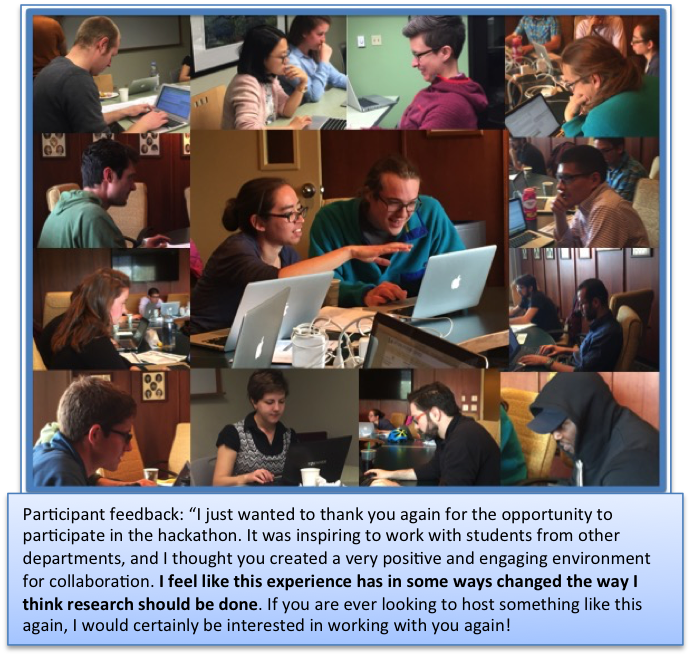
\includegraphics[width =
0.6\textwidth]{figures/csu_hackathon.png} \caption{Some of the approximately 15
undergraduate students, graduate students, postdoctoral fellows, and professors
who participated in a two-day Weather Data Hackathon at Colorado State
University in April 2016 led by Dr. Anderson.} \label{csu-r-hackathon}
\end{SCfigure}

\begin{quotation} ``Applications must include a plan for evaluating the
activities supported by the award in terms of their \textbf{frequency of use}
and their \textbf{usefulness}. The use of \textbf{multiple evaluation
approaches} is highly encouraged as is \textbf{testing several groups with
different characteristics}. The application must specify \textbf{baseline
metrics (e.g., numbers, educational levels, and demographic characteristics of
test group)} in a structured format, as well as \textbf{measures to gauge the
short and long-term success of the research education award in achieving its
objectives}. Applicants are expected to \textbf{obtain feedback from test group}
to help identify weaknesses and to provide suggestions for improvements, and
\textbf{make the evaluation and feedback data} available to NIGMS staff."
\end{quotation}

For each of the modules, we have outlined \textbf{learning objectives} will help us evaluate if the training modules are achieving their educational goals.

\textbf{Evaluation methods}:

\begin{itemize}
\item Google Analytics for online book's website.
\item YouTube analytics for the embedded videos. 
\item Quiz for some modules. Use to evaluate how well they've mastered the material. Use Google Forms to embed these quizzes.
\item Link to voluntary survey in each chapter of the online book: Educational level, demographic characteristics. Includes rating for the usefulness of that module.
\end{itemize}

\begin{table}[!h]

\caption{\label{tab:}\label{tab:evaluation} Pilot testing and evaluation of different groups.}
\centering
\fontsize{8}{10}\selectfont
\begin{tabular}[t]{>{\centering\arraybackslash}p{30em}>{\centering\arraybackslash}p{5em}>{\centering\arraybackslash}p{5em}>{\centering\arraybackslash}p{5em}>{\centering\arraybackslash}p{5em}}
\toprule
\rotatebox{45}{} & \rotatebox{45}{CSU pilot testers} & \rotatebox{45}{Non-CSU pilot testers} & \rotatebox{45}{AAM workshop participants} & \rotatebox{45}{Online users}\\
\midrule
\addlinespace[0.3em]
\multicolumn{5}{l}{\textbf{Characteristics of the trainees?}}\\
\hspace{1em}\tabitem Demographics & \cellcolor{pink}{Yes} & \cellcolor{pink}{Yes} & \cellcolor{pink}{Yes} & \cellcolor{pink}{Yes}\\
\hspace{1em}\tabitem Highest educational degree & \cellcolor{pink}{Yes} & \cellcolor{pink}{Yes} & \cellcolor{pink}{Yes} & \cellcolor{pink}{Yes}\\
\hspace{1em}\tabitem Research role (e.g., principal investigator, research associate, graduate student) & \cellcolor{pink}{Yes} & \cellcolor{pink}{Yes} & \cellcolor{pink}{Yes} & \cellcolor{pink}{Yes}\\
\addlinespace[0.3em]
\multicolumn{5}{l}{\textbf{How often the training materials are used}}\\
\hspace{1em}\tabitem How many trainees have accessed online book? & \cellcolor{pink}{Yes} & \cellcolor{white}{No} & \cellcolor{pink}{Yes} & \cellcolor{white}{No}\\
\hspace{1em}\tabitem How are online book users distributed across the U.S.? & \cellcolor{pink}{Yes} & \cellcolor{white}{No} & \cellcolor{pink}{Yes} & \cellcolor{white}{No}\\
\hspace{1em}\tabitem How many international trainees have accessed the online book? & \cellcolor{pink}{Yes} & \cellcolor{white}{No} & \cellcolor{pink}{Yes} & \cellcolor{white}{No}\\
\hspace{1em}\tabitem How many trainees attended the associated workshop? & \cellcolor{pink}{Yes} & \cellcolor{white}{No} & \cellcolor{pink}{Yes} & \cellcolor{white}{No}\\
\hspace{1em}\tabitem How many trainees attended on-campus CSU piloting? & \cellcolor{pink}{Yes} & \cellcolor{white}{No} & \cellcolor{pink}{Yes} & \cellcolor{white}{No}\\
\hspace{1em}\tabitem How many non-CSU pilot testers participated? & \cellcolor{pink}{Yes} & \cellcolor{white}{No} & \cellcolor{pink}{Yes} & \cellcolor{white}{No}\\
\addlinespace[0.3em]
\multicolumn{5}{l}{\textbf{Patterns in use of each module}}\\
\hspace{1em}\tabitem How long do trainees stay on the webpage for the module? & \cellcolor{pink}{Yes} & \cellcolor{white}{No} & \cellcolor{pink}{Yes} & \cellcolor{white}{No}\\
\hspace{1em}\tabitem For each module video, how often has it been watched? & \cellcolor{pink}{Yes} & \cellcolor{white}{No} & \cellcolor{pink}{Yes} & \cellcolor{white}{No}\\
\hspace{1em}\tabitem When trainees watch a module's video, on average what percent do they watch? & \cellcolor{pink}{Yes} & \cellcolor{white}{No} & \cellcolor{pink}{Yes} & \cellcolor{white}{No}\\
\hspace{1em}\tabitem How often are additional educational materials (quizzes, applied exercise materials) used? & \cellcolor{pink}{Yes} & \cellcolor{white}{No} & \cellcolor{pink}{Yes} & \cellcolor{white}{No}\\
\hspace{1em}\tabitem How often is the entire book downloaded as a PDF or EPUB file? & \cellcolor{pink}{Yes} & \cellcolor{white}{No} & \cellcolor{pink}{Yes} & \cellcolor{white}{No}\\
\hspace{1em}\tabitem Which of the modules are used most frequently? & \cellcolor{pink}{Yes} & \cellcolor{white}{No} & \cellcolor{pink}{Yes} & \cellcolor{white}{No}\\
\addlinespace[0.3em]
\multicolumn{5}{l}{\textbf{Usefulness of each module}}\\
\hspace{1em}\tabitem What were the trainee's goals in using this training material? & \cellcolor{pink}{Yes} & \cellcolor{white}{No} & \cellcolor{pink}{Yes} & \cellcolor{white}{No}\\
\hspace{1em}\tabitem Did this module provide the trainee novel information? & \cellcolor{pink}{Yes} & \cellcolor{white}{No} & \cellcolor{pink}{Yes} & \cellcolor{white}{No}\\
\hspace{1em}\tabitem Does the trainee plan to change research practices based on having taken the module? & \cellcolor{pink}{Yes} & \cellcolor{white}{No} & \cellcolor{pink}{Yes} & \cellcolor{white}{No}\\
\hspace{1em}\tabitem Is so, how does the trainee plan to change research practices based on having taken the module? & \cellcolor{pink}{Yes} & \cellcolor{white}{No} & \cellcolor{pink}{Yes} & \cellcolor{white}{No}\\
\hspace{1em}\tabitem Was the module useful enough that the trainee would recommend it to other scientists? & \cellcolor{pink}{Yes} & \cellcolor{white}{No} & \cellcolor{pink}{Yes} & \cellcolor{white}{No}\\
\hspace{1em}\tabitem Which elements of the training modules (video lecture, written text, additional educational materials) did the trainee find most useful? & \cellcolor{pink}{Yes} & \cellcolor{white}{No} & \cellcolor{pink}{Yes} & \cellcolor{white}{No}\\
\hspace{1em}\tabitem For each module video, are there spots where it is common for trainees to stop watching? & \cellcolor{pink}{Yes} & \cellcolor{white}{No} & \cellcolor{pink}{Yes} & \cellcolor{white}{No}\\
\hspace{1em}\tabitem Why did the trainee chose which modules to use? & \cellcolor{pink}{Yes} & \cellcolor{white}{No} & \cellcolor{pink}{Yes} & \cellcolor{white}{No}\\
\tabitem For the modules taken, what content did the trainee wish had been covered but was not? & \cellcolor{pink}{Yes} & \cellcolor{white}{No} & \cellcolor{pink}{Yes} & \cellcolor{white}{No}\\
\bottomrule
\end{tabular}
\end{table}


\textbf{Groups for piloting and evaluation:}

\begin{itemize}
\item \textbf{Final users of the online book and videos.} These could potentially be from anywhere in the world, and for many we won't have great ways to contact them. 
\item \textbf{Workshop attendees for the workshops we plan to propose and do at national microbiology / immunology conferences.} For these people, we could definitely do a survey before to get information on demographics, education level, interest in the training materials, etc. We could also do a post survey to find out what they learned, how helpful it was, what they found confusing, etc. Finally, we could get their email addresses to ask some longer-term evaluation questions (e.g., How are they using what they learned 1--2 years after taking the workshop? How much did they retain in terms of principals, implementation, and examples?). We can also use questions that are asked during the workshops and areas where additional materials (applied exercises, quizzes, discussion questions) are problematic to help us hone our training materials.
\item \textbf{Early online users.} We will plan to develop and post the text and some of the additional educational materials (e.g., quizzes, discussion questions) online through GitHub \textit{as we write the book and develop the materials}. We will use social media to invite people to try out the book as we develop it. Based on previous work developing online books, we have found that this open development process can help attract users very early in the process, and that these users are often very helpful in providing feedback as the book is developed. We will elicit their feedback through GitHub (``Issues" page will be the main forum for them to post comments and suggestions).
\item \textbf{CSU pilot users.} We can ask these pilot users many questions, both before and after the pilot testing. Further, we will have access to ask them longer-term outcomes, as well as to ask at the department level how the use of these training materials by a number of people in the department has changed research practices and what is considered ``best practice" for research in the department (i.e., a `bubble up" effect).
\item \textbf{Pilot users from other institutions.} Similar to CSU pilot users, although we'll have a bit less access for determining longer-term and department-wide outcomes.
\end{itemize}
    
Examples of what we hope to learn from each group in pilot testing and evaluation (Tables \ref{tab:evaluation}).

\subsection{Dissemination Plan}

We will use GitHub's free ``Pages" website hosting to publish the book freely online, with all materials published under the Creative Commons Attribution-ShareAlike 4.0 International License [ref], \textbf{making all materials freely accessible, both nationally and internationally}. From the beginning of the project, we will publish the book online as it develops, and we will promote this material through postings on social media (e.g., Twitter) and take advantage of our network of colleagues in biomedical research and the R programming community to help promote the availability of the materials (for example, see letter of support from Dr. Peng). This book will be hosted on a ``Git Pages" webpage, allowing the online book to be easily accessed through a link posted on the NIGMS's \textit{Clearinghouse for Training Modules to Enhance Data Reproducibility}. There will be no paywall or other restriction on accessing any of the training materials, and source code for the book and exercises will be published on GitHub. All video and audio content will be published online in free formats through YouTube and SoundCloud, with the content embedded in the online books webpage. At the end of project years 2 and 3, we will also post a static version of the book to the website \textit{bookdown.org}, where people can go to find free online books published using the bookdown format and which invites direct submissions from authors that have used these framework. The PI has previously had substantial success in disseminating online training materials. She is the co-instructor of a five-course specialization on \textit{Mastering Software Development in R} through the Massive Open Online Course platform Coursera. This series has had over 50,000 participants since it was opened in Fall 2016, and an accompanying online book on the LeanPub platform has been downloaded by over 14,000 people.

In addition to these methods of disseminating the training materials to a general audience, \textbf{we will also take specific steps to make sure that our target audience---laboratory-based biomedical scientists---are aware of these training materials.} We will apply to present posters or oral presentations in years 2 and 3 of the project at three national and international conferences (American Society for Microbiology Conference, American Association of Immunologists Meeting, and International Society for the Advancement of Cytometry) to pilot the training materials and help get out the news among our target audience that these materials are freely available. We will also apply to present a workshop in year 2 of the project at the American Society for Microbiology Conference to pilot the training materials and help get out the news among our target audience that these materials are freely available. We will pilot our training materials among CSU researchers in our target audience through biannual, day-long user testing; in addition to providing us with feedback to help refine our materials, this will help us let members of our target audience know that these training materials are freely available and how to find them. We will also invite colleagues (and their research group members) at outside of CSU to serve as early pilot testers of the online version of all our materials. In addition to providing us with feedback to help refine our materials, this will help us let members of our target audience know that these training materials are freely available and how to find them. Finally, we will write and submit a paper describing these training materials and highlighting their content in a biomedical journal relevant to our target audience, like [example of a couple of journals].

\subsection{Timeline}

\begin{figure}[ht]
    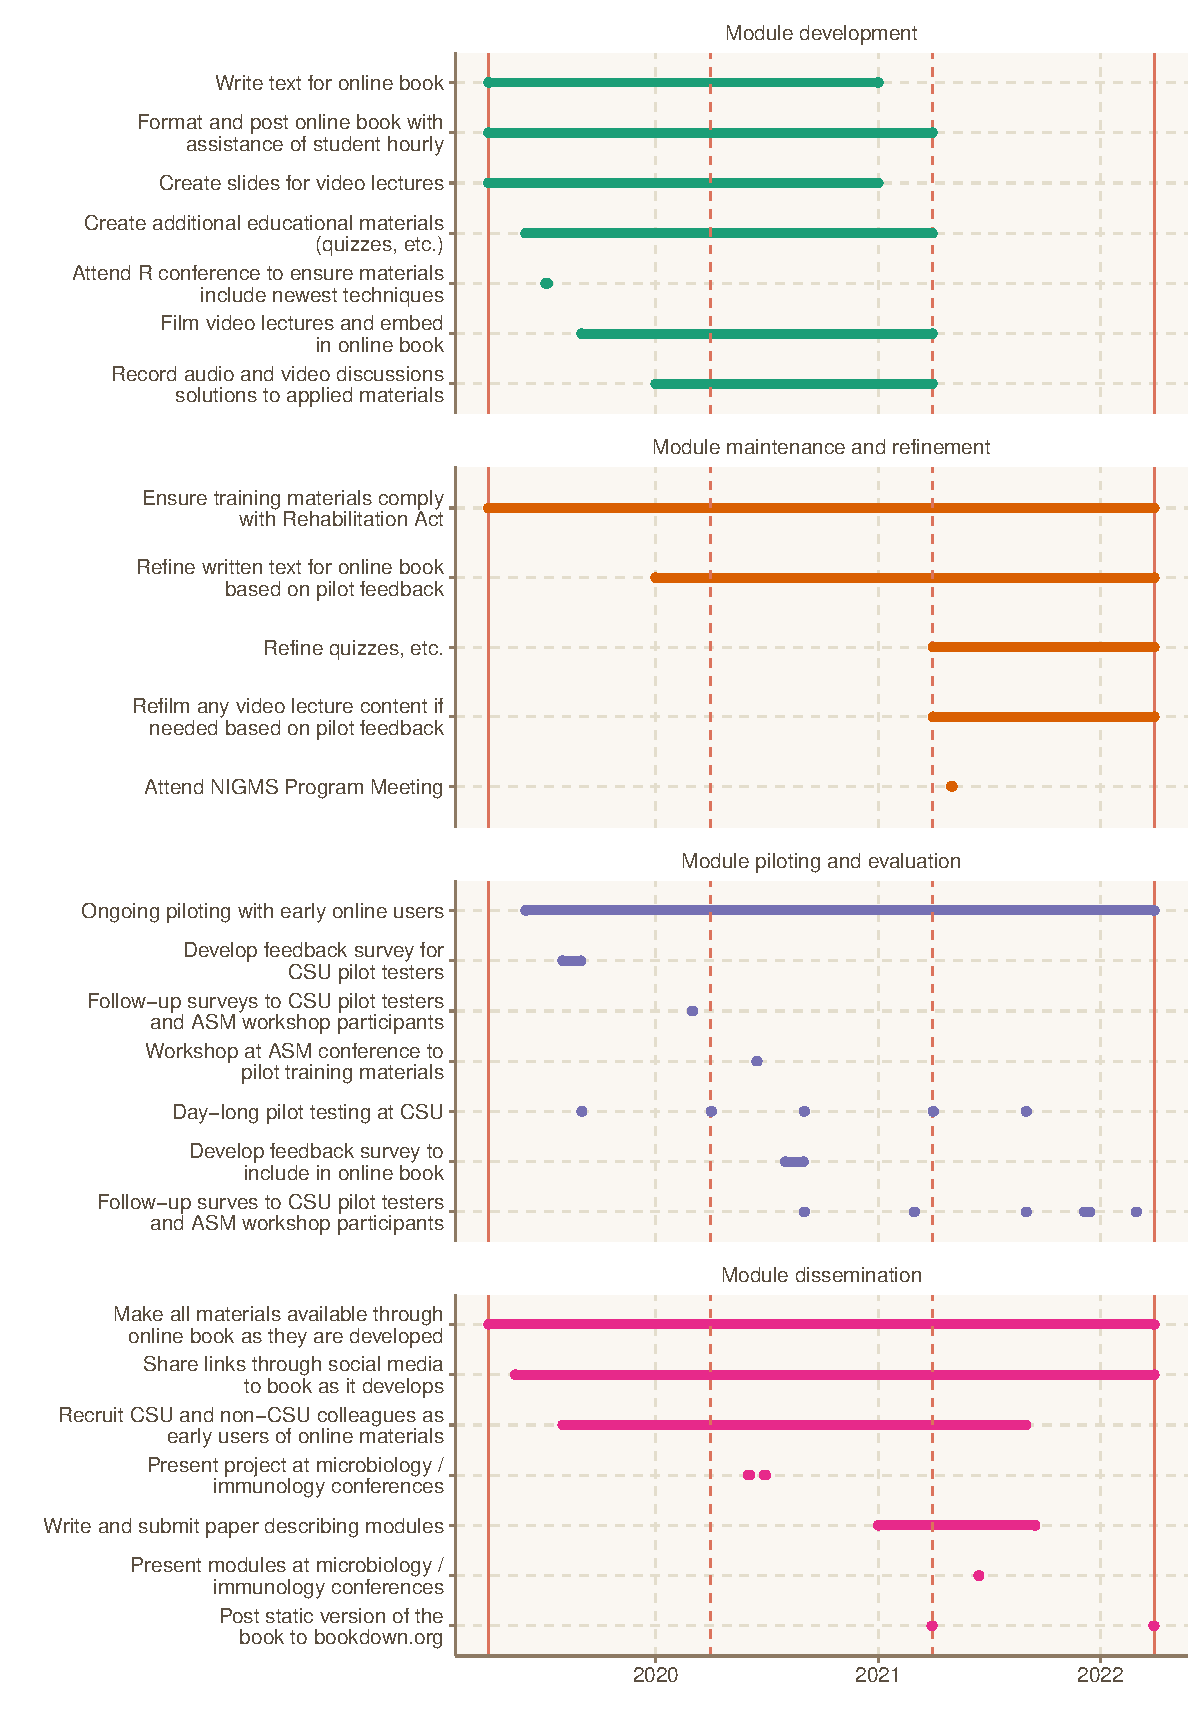
\includegraphics[width=\textwidth]{figures/timeline.pdf}
    \caption{Timeline for proposed activities for this project.}
    \label{fig:timeline}
\end{figure}

\clearpage

\bibliographystyle{unsrtnat}
\bibliography{rep_modules}

\end{document}
